\documentclass[journal,10pt]{IEEEtran}

\usepackage[utf8]{inputenc}
\usepackage[T1]{fontenc}
\usepackage{amsmath,amssymb,amsfonts}
\usepackage{algorithmic}
\usepackage{algorithm}
\usepackage{array}
\usepackage{booktabs}
\usepackage{graphicx}
\usepackage{textcomp}
\usepackage{xcolor}
\usepackage{tikz}
\usepackage{pgfplots}
\usetikzlibrary{positioning,arrows.meta,calc,shapes.geometric,fit,backgrounds,decorations.pathreplacing}
\pgfplotsset{compat=1.18}
\usepackage[colorlinks=true,linkcolor=black,citecolor=blue,urlcolor=blue]{hyperref}
\usepackage{orcidlink}
\usepackage{cleveref}

\hyphenation{op-tical net-works semi-conduc-tor}

% Math shortcuts
\newcommand{\bp}{\mathbf{p}}
\newcommand{\bs}{\mathbf{s}}
\newcommand{\rs}{R_s}
\newcommand{\Rf}{R_f}
\newcommand{\Pe}{P_{\mathrm{err}}}
\newcommand{\Pc}{P_{\mathrm{corr}}}
\newcommand{\Psift}{P_{\mathrm{sift}}}
\newcommand{\Eh}{\mathbb{E}_{h_a}}
\newcommand{\QBER}{\mathrm{QBER}}
\newcommand{\mubold}{\boldsymbol{\mu}}
\newcommand{\todo}[1]{{\color{red}\textbf{TODO: #1}}}

\begin{document}
% R3-5: tat ky hieu '------' thay ten tac gia lap lai; phan bien doc thanh THIEU TEN
\bstctlcite{IEEEexample:BSTcontrol}


\title{KAN-Based Adaptive Parameter Control for\\ Multi-User Satellite FSO/QKD Systems}

\author{%
  Phuc Hao Do~\orcidlink{0000-0003-0645-0021},~\IEEEmembership{Member,~IEEE,}
  Minh Q. Vu~\orcidlink{0000-0001-5054-1794},
  and~Ngoc T. Dang~\orcidlink{0000-0001-9228-5629},~\IEEEmembership{Senior~Member,~IEEE}%
  \thanks{P. H. Do is with the Faculty of Information Technology, Da Nang Architecture University, Da Nang, Vietnam (e-mail: haodp@dau.edu.vn). \emph{(Corresponding author: Phuc Hao Do.)}}%
  \thanks{M. Q. Vu and N. T. Dang are with the Faculty of Telecommunications, Posts and Telecommunications Institute of Technology, Hanoi 100000, Vietnam (e-mail: minhvq@ptit.edu.vn; ngocdt@ptit.edu.vn).}%
}

\markboth{IEEE Transactions on Communications, Vol.~XX, No.~YY, 2026}{Do \MakeLowercase{\textit{et~al.}}: KAN-Based Adaptive QKD}

\maketitle

% ⛔ HAN CUA TCOM, nguyen van tai comsoc.org/publications/journals/ieee-tcom/policies-and-guidelines:
%   "It is essential that each manuscript be accompanied by a 75- to 200-word abstract
%    clearly outlining the scope and contributions of the paper"
% Ban v1 da nop la 219 tu (da vuot 19), ban R1 phong len 306 roi 350. Dem bang
%   python3 scripts/kiem_dinh_dang_tcom.py
% truoc MOI lan dung goi. Khong duoc noi them mot menh de vao day ma khong dem lai.
For multi-user satellite free-space-optical quantum key distribution with
subcarrier-intensity-modulation BPSK and dual-threshold detection, we optimize
modulation depth, dual-threshold coefficients and the inter-user exclusion ratio under
unauthorized-receiver and beam-splitting security, a nonconvex problem coupling all $N$ pairs. A two-level decomposition with an exact
outer/inner split is the oracle for a learned controller:
Kolmogorov--Arnold Networks (KAN), regularized perceptrons (MLP), linear map. Over an SGP4-propagated Walker shell at Hanoi, adaptation yields $2.10\times$
the key and $3.6\times$ the secure pair-time; over $\rSparseEpochs$ epochs on a
sparser shell the static baseline yields $\rSparseStatLo$ to $\rSparseStatHi$ secure
pair-steps against $\rSparseAdaptLo$ to $\rSparseAdaptHi$ for adaptation: survival, not
operation. Three of four outputs are constant (the
modulation depth saturates), so accuracy is reported on the one with signal.
In the cluster setting KAN attains $0.010\pm0.001$ against $0.018\pm0.022$ for the MLP at $43\%$
of its parameters, though a paired test does not establish it ($p=0.29$): the gap comes
from $2$ of $20$ seeds where the MLP returns the linear fit. Retention saturates for
all three and is not ranked. What separates them is parameter count and the
closed-form rule extractable from the KAN, post-extraction $R^2 \approx 0.97$ in the
single-link setting, at a latency cost.


\noindent\textbf{Reproducibility.} All code, bundled TLE data, and run scripts that reproduce every figure and table in this paper are available at \url{https://github.com/haodpsut/kan-satellite-fso-qkd}; the headline runs reproduce in under one hour on a single CPU plus an RTX-class GPU for the KAN training phase.

\begin{IEEEkeywords}
Quantum key distribution, free-space optical communications, satellite networks, Kolmogorov--Arnold Networks, multi-user QKD, adaptive control.
\end{IEEEkeywords}

\section{Introduction}\label{sec:intro}

\IEEEPARstart{S}{atellite}-based free-space optical (FSO) channels are the most credible medium for intercontinental quantum key distribution (QKD): they avoid the exponential photon-loss bound of optical fiber and exploit the near-vacuum of space for low excess noise \cite{liao2017micius,bedington2017progress,sidhu2021advances,pirandola2020advances}. The 2017 demonstration of decoy-state BB84 between the Micius satellite and ground stations in China \cite{liao2017micius}, the simultaneous entanglement distribution at $1{,}200$ km baseline \cite{yin2017satellite}, and the relayed intercontinental key exchange of \cite{liao2018satellite} together establish satellite QKD as a near-term technology rather than a research curiosity. Recent progress is summarized in \cite{sidhu2021advances,pirandola2020advances}. Two reviews frame the present work in particular: \cite{xu2020rmp} surveys how device imperfections, rather than protocol design, set the security of practical QKD, which is the regime our parameter-control problem lives in; and \cite{lu2022micius} reviews the Micius programme, still the only satellite platform on which these protocols have been demonstrated end to end, and the source of the link budgets that make a multi-user relay architecture worth optimizing at all.

Among the QKD families adapted to FSO, the subcarrier-intensity-modulation BPSK with dual-threshold direct detection (SIM-BPSK/DT-DD) scheme proposed by Vu, Pham, Dang, Le, and Pham \cite{vu2020access,vu2022access,vu2023photonics} is attractive because it relies on entirely classical components (an EDFA-amplified GEO source, PIN photodetectors, and dual-threshold post-processing), yet is reported in \cite{vu2020access,vu2022access,vu2023photonics} to admit a positive secret-key rate against unauthorized-receiver attacks (URA) and beam-splitting attacks (BSA) \cite{lutkenhaus1999estimates,huttner1995quantum}, provided that the modulation depth $\mu$, the DT scale coefficients $\beta_A, \beta_i$, and the multi-user fading-randomness exclusion ratio $\chi$ are appropriately chosen. We state the scope of that guarantee precisely, because the present work inherits it rather than re-deriving it: the secret-key rate used throughout this paper is the asymptotic Csisz\'ar--K\"orner fraction $\max\{0, H_2(P_e) - H_2(\mathrm{QBER})\}$ per sifted bit, evaluated against the two attack models above. It carries no finite-key correction, no composable-security statement, and no claim of optimality against general coherent attacks; it is a sufficient-condition surrogate that we optimize, not a security proof that we establish. SIM-BPSK is well established for classical FSO links \cite{popoola2009bpsk,kaushal2017fso}, and DT-DD inherits its noise-budget structure from the standard outage-capacity analysis \cite{farid2007outage,sandalidis2008ber}.

The three papers in the lineage establish, in increasing generality, the relay-assisted single-link case \cite{vu2020access}, the entanglement-based two-user case \cite{vu2022access} (which adapts the BBM92 protocol \cite{bbm92} to the DT/DD measurement basis), and the GEO source serving $N$ ground users via dual LEO relays with a closed-form inclusion-exclusion term \cite{vu2023photonics}. In all three, the parameters $(\mu, \beta, \chi)$ are picked \emph{statically}: a single operating point is selected by reading the analytic performance plots at a representative geometry, and that point is then held throughout operation.

We show in this paper that for the realistic case of a LEO relay traversing its pass while serving an asymmetric cluster of ground users, the static-parameter assumption is the dominant performance bottleneck. Peak elevation, slant range, log-amplitude turbulence variance \cite{andrews2005laser,vetelino2007fade}, and the URA leakage geometry vary by orders of magnitude across a single 5 to 10 minute pass, and the optimal $\bp(t) = (\mu, \beta_A, \{\beta_i\}, \chi)$ drifts continuously with the time-varying state $\bs(t)$. Under realistic constellations propagated from real Two-Line Elements (TLE) via the SGP4 propagator \cite{hoots1980sgp4,vallado2006sgp4} on Starlink-density shells \cite{del2019leosat,leyva2021inter}, we further show that \emph{no} single static $\bp$ produces any secure pair-step over a typical $90$-minute observation window, so adaptation is a precondition for the system to operate at all rather than a marginal improvement.

The modulation-signalling branch of QKD that this paper belongs to has moved on since the three papers above, and in directions that sharpen what is and is not new here. Subcarrier-wave QKD has been analysed numerically for free-space ship-to-port links \cite{goncharov2025scw} and routed through a deployed metropolitan transport network \cite{tarabrina2023scw}, which establishes the signalling format outside the laboratory but in both cases for a \emph{single} link rather than a shared relay. On the transmitter side, direct intensity and phase modulation has been demonstrated as a QKD source \cite{liu2026intensity}, which is the hardware assumption our modulation depth parameterizes. The free-space continuous-variable line is surveyed in \cite{kargina2026cvqkd}; it shares our reliance on classical coherent components but replaces the dual-threshold decision with homodyne detection, so the parameter that dominates our problem, a detection threshold, has no counterpart there. What none of these address is the coupling we study: a single global modulation depth that every user in a cluster must share.

Learning-based parameter control for QKD is itself an active line, and the closest neighbour to this work is \cite{mohamed2026aml}, which couples a temporal convolutional forecaster with a proximal-policy-optimization agent to retune decoy intensities online for BB84, E91 and COW while keeping a composable-security constraint. The contrast is instructive in three ways. First, the physical layer differs: that work tunes photon-counting discrete-variable protocols, whereas the parameters here are a modulation depth and a pair of detection thresholds in an intensity-modulated direct-detection link, so the two parameter spaces do not overlap and a numerical head-to-head comparison would compare protocols rather than controllers. Second, that work is single-link; the coupling that makes the present problem hard, a single global modulation depth shared by every Alice-Bob pair in a cluster, does not arise there. Third, it learns online by reinforcement while we learn offline by supervision from a decomposed oracle, which buys determinism and an inspectable target at the cost of needing that oracle. A reinforcement-learning controller for the multi-user FSO setting is a worthwhile comparison that we leave to future work; building a fair one is a study in itself, and a weak re-implementation would be worse evidence than none.

\subsection{Contributions}

This paper makes the following contributions:

\begin{enumerate}
\item \textbf{Full multi-user joint problem.} We restate the GEO/multi-LEO/$N$-user system of \cite{vu2023photonics} together with the pointing-error/Gaussian-beam model of \cite{vu2020access} (dropped in \cite{vu2023photonics}) and derive the corresponding joint problem \textbf{(P)} over $\bp=(\mu, \beta_A, \{\beta_i\}, \chi)$ with URA, BSA, and an inter-user secrecy constraint. The problem is nonconvex with three sources of coupling: $\mu$ shared globally, $\chi$ entering every pair through a product field $\phi_i = \prod_{j\neq i}(1-P_c^j)$, and $\beta_A$ shared between Alice and every Bob. The inclusion--exclusion term of \cite[Eq.~22]{vu2023photonics} is generalized to asymmetric clusters in closed form.
\item \textbf{Principled two-level decomposition.} We expose the variable roles to obtain a two-level decomposition whose outer/inner split is exact (a relaxation-free reformulation of \textbf{(P)}): an outer two-dimensional search over $(\mu,\chi)$ wraps an inner mean-field block-coordinate solver over the thresholds. The symmetric-cluster fixed point provably recovers \cite[Eq.~24]{vu2023photonics}, and the decomposition matches a brute-force joint grid optimum on a two-user cluster to four decimals.
\item \textbf{Two-stage controller with KAN.} The decomposed oracle generates supervised pairs $(s(t)\!\to\!p^\star(t))$ for a two-stage controller: a global head consumes cluster-aggregate features and predicts $(\mu, \chi, \beta_A)$; a per-user shared head consumes $(s_i, \beta_A, \mu, \chi)$ and predicts $\beta_i$. We compare a Kolmogorov--Arnold Network (KAN) \cite{liu2024kan,liu2024kan2} against a regularized multi-layer perceptron and a linear residual baseline on a five-axis trade-off (regression accuracy, closed-loop secret-key retention, parameter count, inference latency, and interpretability). Deep learning for the classical physical layer \cite{oshea2017introduction,wang2017deep,ye2018deep} and reinforcement-learning control \cite{luong2019applications} are well studied; KAN is attractive here because its spline activations admit symbolic extraction \cite{liu2024kan2,cranmer2020discovering}, which yields a closed-form rule for $\beta^\star$.
\item \textbf{TLE-driven realistic-orbit validation.} An SGP4 path mirrors the analytic-orbit API so every script accepts \texttt{--tle} as a drop-in switch, with a synthetic Walker shell reproducing Starlink coverage statistics offline and a Celestrak bundle loadable via \texttt{--tle PATH}. Over a Hanoi ground station, the static baseline collapses to zero secure pair-steps on the Walker constellation, while the adaptive controller recovers a non-trivial fraction near overhead.
\item \textbf{Honest multi-axis evaluation.} We report results with explicit mean$\pm$std over five seeds, fair (regularized) MLP baselines, and a model-agnostic $\beta$ safety-margin recipe that lifts feasibility by 1.1--1.5$\times$ for every controller. KAN does not dominate every axis; its value is parameter efficiency plus an interpretable closed-form rule for $\beta$ with symbolic $R^2 \approx 0.97$. We disclose where the symbolic extraction fails (the $\mu^\star$ saturation regime), where the controllers transfer (single-link) and where they do not (multi-user cluster, the residual-learning rescue), and how the design generalizes to real-orbit operation.
\end{enumerate}

\section{System Model}\label{sec:system}

\subsection{Architecture}\label{sec:system:arch}

A geostationary source \emph{Charlie} ($C$) at altitude $H_C{=}35\,793$~km broadcasts a SIM-BPSK--modulated continuous-wave laser of mean power $P{=}32$~dBm and wavelength $\lambda{=}1550$~nm. The signal is amplify-and-forward relayed by two low-Earth-orbit satellites ($H_L{=}550$~km, Starlink shell) acting as optical amplifiers (EDFA gain $G_a{=}40$~dB). The relayed beam illuminates a ground cluster consisting of a single server \emph{Alice} ($A$) and $N$ users \emph{$B_1,\dots,B_N$}; an entanglement-based BBM92-style key is then established \emph{per pair} $(A,B_i)$ using only classical optical components and dual-threshold post-processing. An eavesdropper \emph{Eve} sits at radial offset $d_E$ from each legitimate receiver. The architecture is depicted in Fig.~\ref{fig:arch}.

\begin{figure*}[!htbp]
\centering
\resizebox{0.92\textwidth}{!}{% System architecture (Fig. 1) -- redrawn for IEEE TCOM, publication grade.
%
% Layout philosophy:
%   * Strict top-down signal flow: Charlie (GEO) -> two LEO EDFA relays ->
%     ground-cluster receivers (Alice + N Bobs).
%   * Adversaries in muted red: URA leakage routed OUTSIDE the cluster down
%     to the Eves; BSA tap drawn at the LEO relay tier.
%   * Controller K to the RIGHT, with action p(t) flowing IN to the relays
%     and state s(t) flowing OUT from the cluster (clean orthogonal routing,
%     no diagonal crossings, no line through a node).
%
% Coordinate grid (cm):
%   Charlie centre (0, 5.4);  LEOs at (-2.6, 3.0) and (2.6, 3.0);
%   Receiver row y=0.3: Alice -3.0, B1 -1.3, dots 0.1, BN 1.5;
%   Eve row y=-1.6 under Alice and B_N;
%   Controller centre (8.6, 1.8);
%   URA verticals at x=-5.1 (left) and x=5.1 (right);
%   s(t) routed under cluster at y=-3.3.
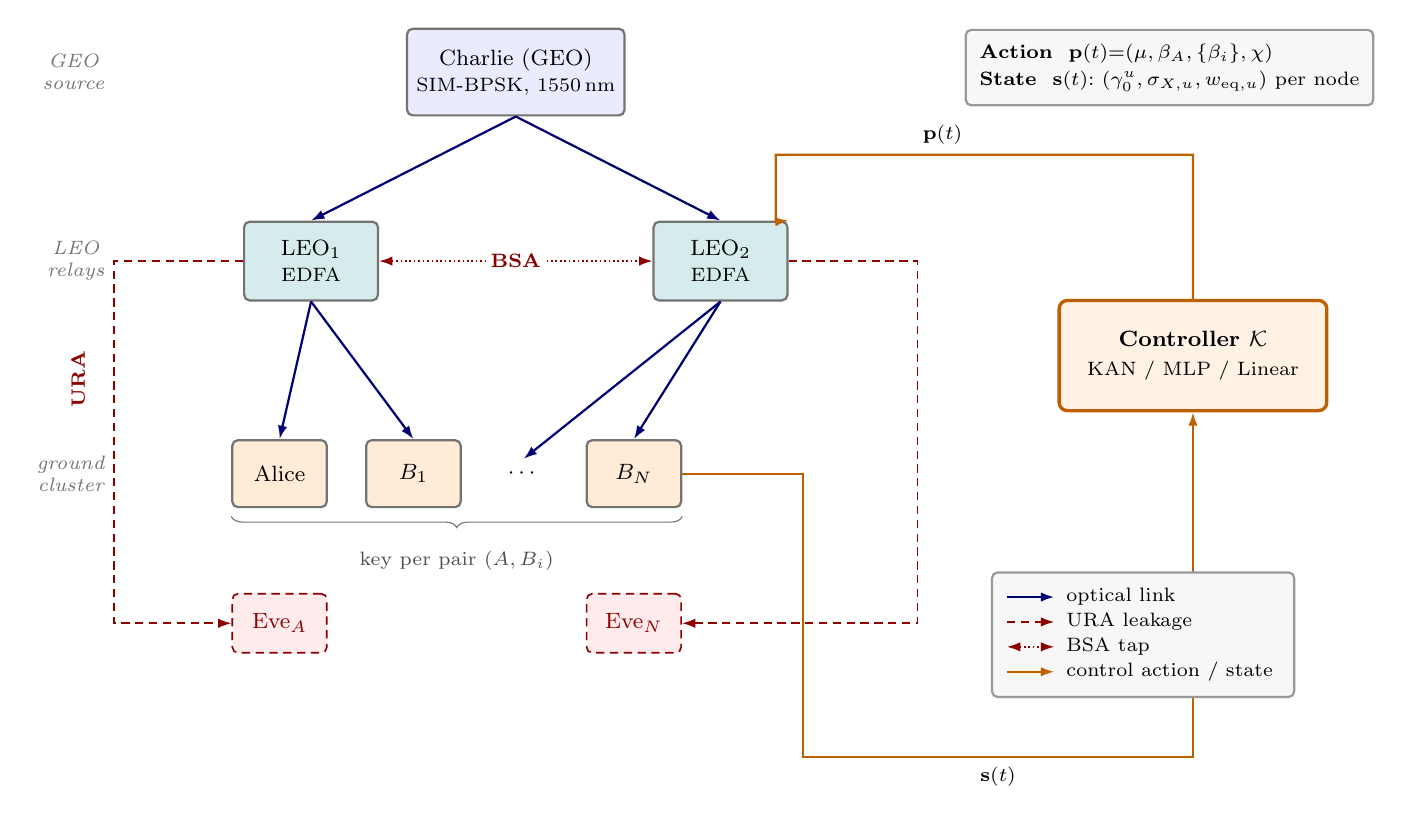
\begin{tikzpicture}[
  font=\footnotesize,
  >={Latex[length=1.7mm,width=1.2mm]},
  %--- node styles (split fill/text/draw; never `color=`) ---
  geo/.style    ={draw=black!55,thick,fill=blue!8,text=black,rounded corners=2pt,
                  minimum width=22mm,minimum height=11mm,align=center},
  leo/.style    ={draw=black!55,thick,fill=teal!16,text=black,rounded corners=2pt,
                  minimum width=17mm,minimum height=10mm,align=center},
  user/.style   ={draw=black!55,thick,fill=orange!16,text=black,rounded corners=2pt,
                  minimum width=12mm,minimum height=8.5mm,align=center},
  eve/.style    ={draw=red!55!black,semithick,fill=red!8,text=red!55!black,
                  rounded corners=2pt,densely dashed,
                  minimum width=12mm,minimum height=7.5mm,align=center},
  ctrl/.style   ={draw=orange!75!black,very thick,fill=orange!10,text=black,
                  rounded corners=3pt,minimum width=34mm,minimum height=14mm,
                  align=center},
  legendbox/.style={draw=black!40,thick,fill=black!3,text=black,rounded corners=2pt,
                  inner sep=5pt,align=left,font=\scriptsize},
  tier/.style   ={text=black!55,font=\scriptsize\itshape,align=center},
  %--- arrow styles ---
  opt/.style    ={->,thick,draw=blue!45!black},
  leak/.style   ={->,semithick,draw=red!55!black,densely dashed},
  bsa/.style    ={<->,semithick,draw=red!55!black,densely dotted},
  ctl/.style    ={->,thick,draw=orange!75!black},
]

%==================== nodes ====================
\node[geo]  (C)  at (0, 5.4) {Charlie (GEO)\\\scriptsize SIM-BPSK, $1550$\,nm};
\node[leo]  (L1) at (-2.6, 3.0) {LEO$_1$\\\scriptsize EDFA};
\node[leo]  (L2) at ( 2.6, 3.0) {LEO$_2$\\\scriptsize EDFA};

\node[user] (A)    at (-3.0, 0.3) {Alice};
\node[user] (B1)   at (-1.3, 0.3) {$B_1$};
\node       (dots) at ( 0.1, 0.3) {$\cdots$};
\node[user] (BN)   at ( 1.5, 0.3) {$B_N$};

\node[eve]  (EA)   at (-3.0,-1.6) {Eve$_A$};
\node[eve]  (EN)   at ( 1.5,-1.6) {Eve$_N$};

\node[ctrl] (K)    at (8.6, 1.8)
  {\textbf{Controller }$\mathcal{K}$\\[1pt]\scriptsize KAN / MLP / Linear};

%==================== tier labels (left margin) ====================
\node[tier,anchor=east] at (-5.1, 5.4) {GEO\\source};
\node[tier,anchor=east] at (-5.1, 3.0) {LEO\\relays};
\node[tier,anchor=east] at (-5.1, 0.3) {ground\\cluster};

%==================== optical links (top-down) ====================
\draw[opt] (C.south) -- (L1.north);
\draw[opt] (C.south) -- (L2.north);
\draw[opt] (L1.south) -- (A.north);
\draw[opt] (L1.south) -- (B1.north);
\draw[opt] (L2.south) -- (dots.north);
\draw[opt] (L2.south) -- (BN.north);

%==================== BSA tap at the relay tier ====================
\draw[bsa] (L1.east) --
   node[fill=white,inner sep=1.5pt,font=\scriptsize\bfseries,text=red!55!black]{BSA}
   (L2.west);

%==================== URA leakage (orthogonal, outside cluster) ====================
\draw[leak] (L1.west) -- (-5.1, 3.0) -- (-5.1, -1.6) -- (EA.west);
\draw[leak] (L2.east) -- (5.1, 3.0) -- (5.1, -1.6) -- (EN.east);
\node[text=red!55!black,font=\scriptsize\bfseries,anchor=south,rotate=90]
  at (-5.35, 1.5) {URA};

%==================== ground-cluster brace ====================
\draw[decorate,decoration={brace,amplitude=4pt,mirror,raise=3pt},draw=black!55]
  (A.south west) -- (BN.south east);
\node[font=\scriptsize,text=black!70,anchor=north]
  at ($(A.south west)!0.5!(BN.south east) + (0,-0.42)$)
  {key per pair $(A,B_i)$};

%==================== control signals ====================
% Action p(t): controller -> relay tier. Routed UP and over the relay row at
% y=4.35 (clear of the URA-L2 stub at y=3.0), then DOWN into LEO_2 top-right,
% offset from the Charlie optical link that enters LEO_2.north.
\draw[ctl] (K.north) -- (8.6, 4.35)
   -- node[above,pos=0.6,font=\scriptsize,text=black]{$\bp(t)$} (3.3, 4.35)
   -- (3.3, 3.5) -- (L2.north east);

% State s(t): from the cluster, down and under, then up into the controller.
\draw[ctl] (BN.east) -| (3.65, -3.3)
   -- node[below,font=\scriptsize,text=black]{$\bs(t)$} (8.6,-3.3)
   -- (K.south);

%==================== legend (bottom-right, clear of routing) ====================
\node[legendbox,anchor=south east] at (9.9, -2.55) {%
  \begin{tabular}{@{}c@{\ \,}l@{}}
    \tikz{\draw[opt]  (0,0) -- (6mm,0);} & optical link\\[1pt]
    \tikz{\draw[leak] (0,0) -- (6mm,0);} & URA leakage\\[1pt]
    \tikz{\draw[bsa]  (0,0) -- (6mm,0);} & BSA tap\\[1pt]
    \tikz{\draw[ctl]  (0,0) -- (6mm,0);} & control action / state
  \end{tabular}
};

%==================== action / state caption (top-right) ====================
\node[legendbox,anchor=north west] at (5.7, 5.95) {%
  \textbf{Action } $\bp(t){=}(\mu,\beta_A,\{\beta_i\},\chi)$\\[2pt]
  \textbf{State } $\bs(t){:}\ (\gamma_0^u,\sigma_{X,u},w_{\mathrm{eq},u})$ per node
};

\end{tikzpicture}
}
\caption{System architecture. A GEO source Charlie broadcasts a SIM-BPSK signal through two LEO EDFA relays to a ground cluster (Alice + $N$ Bobs); the secret key is established per pair $(A,B_i)$. An eavesdropper Eve at offset $d_E$ from each receiver mounts an unauthorized-receiver attack (URA); a beam-splitter at the LEO relay mounts a beam-splitting attack (BSA). The proposed controller selects $\bp(t) = (\mu, \beta_A, \{\beta_i\}, \chi)$ from the time-varying cluster state $\bs(t)$.}
\label{fig:arch}
\end{figure*}

\subsection{Channel Model}\label{sec:system:channel}

The end-to-end channel coefficient for any link $C\to U$ ($U\in\{A,B_i,E\}$) factors as
\begin{equation}
  h_{e2e}^U = h_g^U\, h_l^U\, h_a^U,
\end{equation}
where the geometric, attenuation, and turbulence components are obtained as follows.

\subsubsection{Gaussian-beam spreading}
At link distance $L$ a beam of waist $w_0 = \lambda/(\pi\theta)$ (divergence $\theta = 2.44\lambda/D$) has radius $w_L = w_0 [1+(\lambda L/(\pi w_0^2))^2]^{1/2}$ \cite{andrews2005laser}. The fraction collected by a receiver aperture of radius $a$ at radial offset $r$ from the footprint center is, after the small-aperture approximation of \cite{farid2007outage},
\begin{align}
  h_g(r) &\approx A_0 \exp\!\Big(-\frac{2r^2}{w_{L,\mathrm{eq}}^2}\Big),\qquad A_0 = [\mathrm{erf}(\upsilon)]^2, \label{eq:hg}\\
  \upsilon &= \frac{\sqrt\pi\,a}{\sqrt2\,w_L},\quad
  w_{L,\mathrm{eq}}^2 = w_L^2\,\frac{\sqrt\pi\,\mathrm{erf}(\upsilon)}{2\upsilon e^{-\upsilon^2}}.\label{eq:weq}
\end{align}
For Eve at $r = d_E$ the geometric leakage ratio $h_g^E/h_g^U = \exp(-2 d_E^2/w_{L,\mathrm{eq}}^2)$ is close to unity for realistic $d_E$ (tens of metres) versus footprint widths of hundreds of metres; security must therefore come from small $\mu$ rather than from geometry alone.

\subsubsection{Atmospheric attenuation}
Beer--Lambert with visibility-dependent attenuation
\begin{equation}
  h_l = e^{-\sigma L_{h\text{-}U}},\quad \sigma(\lambda) = \frac{3.912}{V}\Big(\frac{\lambda[\mathrm{nm}]}{550}\Big)^{-q(V)},
\end{equation}
where $L_{h\text{-}U} = (H_h - H_U)/\cos\theta_U$, $H_h{=}20$~km, and the size-distribution coefficient is the standard piecewise law $q(V) = 1.6$ for $V > 50$~km, $q(V) = 1.3$ for $6 < V \le 50$~km, and $q(V) = 0.585\,V^{1/3}$ for $V \le 6$~km.

\subsubsection{Log-normal turbulence}
For elevations $\ge 30^\circ$ (zenith $\le 60^\circ$) the turbulence is weak and $h_a$ is log-normal with unit mean \cite{andrews2005laser,vetelino2007fade}: $f_{h_a}(h_a) = \tfrac{1}{\sqrt{8\pi}\,h_a\,\sigma_X}\exp(-(\ln h_a - 2\mu_X)^2/(8\sigma_X^2))$ with $\mu_X = -\sigma_X^2$ enforcing $\mathbb{E}[h_a] = 1$. The log-amplitude variance is the (quarter-)Rytov variance
\begin{equation}
  \sigma_X^2 = 0.56\,k^{7/6}\sec^{11/6}(\theta_U)\int_{H_U}^{H_C} C_n^2(h)(h-H_U)^{5/6}dh,
\end{equation}
with the Hufnagel--Valley profile $C_n^2(h) = 0.00594(w/27)^2(10^{-5}h)^{10}e^{-h/1000} + 2.7\times10^{-16}e^{-h/1500} + C_n^2(0)e^{-h/100}$ and $k = 2\pi/\lambda$.

\subsection{Detection in Reduced Form}\label{sec:system:detection}

Define the deterministic mean peak signal current
\begin{equation}
  s^U = \tfrac14 \mu R_e P G_a \bar h^U,\quad \bar h^U = h_g^U h_l^U,
\end{equation}
and the normalized mean SNR amplitude $\gamma^U \triangleq s^U/N^U$, where $(N^U)^2$ is the AWGN variance budgeted in \cite[Eq.~4]{vu2023photonics} (shot, background, ASE, thermal). For the DT scale coefficient $\beta^U$, the conditional probabilities collapse to two log-normal expectations
\begin{align}
  \Pc^U &= \Eh\!\big[ Q(\beta^U + \gamma^U(1-h_a))\big], \label{eq:pc}\\
  \Pe^U &= \Eh\!\big[ Q(\beta^U + \gamma^U(1+h_a))\big], \label{eq:pe}
\end{align}
both evaluated by Gauss-Hermite quadrature with $h_a(x_j) = \exp(2\sqrt2\sigma_X x_j - 2\sigma_X^2)$ \cite[Eq.~30]{vu2023photonics}; the order-$n$ nodes and weights are tabulated in \cite[Tbl.~25.10]{abramowitz1965handbook}, and $n{=}20$ converge to numerical precision for the values of $\sigma_X$ encountered along a LEO pass. The per-link sift probability and QBER follow as $\Psift^U = \Pc^U + \Pe^U$ and $\QBER^U = \Pe^U/\Psift^U$.

\subsection{Pairwise Sift, Exclusion, and Secret Key Rate}\label{sec:system:pair}

For the pair $(A,B_i)$ the raw sift is $P^{AB_i} = \Psift^A \Psift^i$ and the QBER is
\begin{equation}
  \QBER^{AB_i} = \frac{\Pc^A \Pe^i + \Pe^A \Pc^i}{\Psift^A \Psift^i}.\label{eq:qber_pair}
\end{equation}
The proposed multiple-access scheme retains only bits not coincidentally accepted by other pairs. Assuming statistically independent acceptance across users (independent per-link fading), inclusion--exclusion over the asymmetric cluster yields the closed-form excluded sift
\begin{equation}
  P^{AB_i}_{\mathrm{excl}} = \Pc^A \Pc^i\Big[1 - \prod_{j\neq i}(1 - \Pc^j)\Big],\label{eq:excl}
\end{equation}
which generalizes the symmetric expression of \cite[Eq.~22]{vu2023photonics}. We verify in the unit tests that \eqref{eq:excl} reproduces a direct subset-enumeration inclusion--exclusion sum to $10^{-12}$ for $N\in\{1,2,4,6\}$. With $\chi\in[0,1]$ controlling the strength of the exclusion,
\begin{equation}
  P^{AB_i}_\chi = P^{AB_i} - \chi P^{AB_i}_{\mathrm{excl}},\qquad \rs^i = P^{AB_i}_\chi R_b.
\end{equation}
The per-pair secret fraction (binary-erasure wiretap, Eve\textsubscript{1} near Alice, Eve\textsubscript{2} near $B_i$) is
\begin{equation}
  \sigma_i = \max\!\big(0,\, I(A;B_i) - \max(I(A;E_1), I(B_i;E_2))\big),\label{eq:sigma}
\end{equation}
with $I(A;B_i) = 1 - H_2(\QBER^{AB_i})$ and $I(U;E) = 1 - H_2(\Pe^E)$. The cluster key rate, the objective of \textbf{(P)}, is
\begin{equation}
  \Rf(\bp;\bs,t) = \sum_{i=1}^N \rs^i\,\sigma_i.\label{eq:Rf}
\end{equation}


\section{Joint Optimization Problem}\label{sec:formulation}

\subsection{Decision Variables and Couplings}

At each time instant $t$ of a LEO pass, the cluster state
\begin{equation}
  \bs(t) = \big(\,s_A(t),\,s_1(t),\dots,s_N(t),\,d_E\,\big)
\end{equation}
is computed from the time-varying geometry via Sec.~\ref{sec:system:channel}; each $s_u = (\gamma_0^u, \sigma_{X,u}, w_{\mathrm{eq},u})$ captures the per-node SNR scale, log-amplitude variance, and beam width. The controller selects
\begin{equation}
  \bp(t) = \big(\mu,\, \beta_A,\, \{\beta_i\}_{i=1}^N,\, \chi\big)
\end{equation}
with $\mu\in(0,1)$, $\beta\in[\beta_{\mathrm{lo}}, \beta_{\mathrm{hi}}]$, and $\chi\in[0,1]$. Three sources of coupling distinguish \textbf{(P)} from a per-link problem:
\begin{itemize}
\item \emph{Global $\mu$.} The modulation depth feeds into every $\gamma^u = \gamma_0^u \mu$ and is the URA security lever ($\Pe^E \to 0.5$ as $\mu\to 0$).
\item \emph{Shared $\beta_A$.} Alice's threshold enters every pair through $\Pc^A$ and $\Pe^A$ in \eqref{eq:qber_pair}; choosing $\beta_A$ to favor one Bob hurts the others.
\item \emph{Field $\chi$.} The exclusion term \eqref{eq:excl} couples every pair through the field $\phi_i = \prod_{j\neq i}(1-\Pc^j)$; binding $\chi$ to enforce inter-user secrecy hurts the asymptotically weakest user the most.
\end{itemize}

\subsection{Threats and Constraints}

Two threats are modeled.

\subsubsection{Unauthorized-Receiver Attack (URA)}
An eavesdropper near each legitimate node uses the optimal decision threshold $\beta^E = 0$ (she cannot know the legitimate $\beta$). Her error probability with her own ratio $\gamma^E = s^E/N^E$ (where $s^E \propto h_g^E$ via \eqref{eq:hg}) is
\begin{equation}
  \Pe^E = \Eh[Q(\gamma^E h_a)].\label{eq:eve}
\end{equation}
As $\mu \to 0$ we have $\gamma^E \to 0$ and $\Pe^E \to Q(0) = 1/2$. The security target is $\Pe^E > p_e^{\min} = 0.1$ \cite[Sec.~V-B]{vu2023photonics}; the same wiretap idea underlies the classical secrecy-rate bound of \cite{wyner1975wiretap}, generalized to the practical-QKD setting in \cite{lutkenhaus1999estimates,scarani2009security}.

\subsubsection{Beam-Splitting Attack (BSA)}
An attacker installs a passive beam splitter at the LEO relay drawing fraction $\eta$ of the optical power; this is the dominant side-channel threat against weak-coherent-state QKD \cite{huttner1995quantum,lutkenhaus1999estimates}. Her presence is detectable as a sift-probability deviation
\begin{equation}
  m_{\mathrm{BSA}}(\beta) = 1 - \frac{\Psift(\gamma(1-\eta_{\mathrm{leak}}))}{\Psift(\gamma)},
\end{equation}
which is monotonically increasing in $\beta$. We require $m_{\mathrm{BSA}}(\beta_A), m_{\mathrm{BSA}}(\beta_i) \ge m^{\min}{=}0.5\%$ at the assumed split $\eta_{\mathrm{leak}}{=}1.5\%$. This pair of numbers sets the \emph{detection sensitivity} of the design, and it is sharper than it looks. Sweeping $\eta_{\mathrm{leak}}$ over the oracle solutions of all $250$ clusters, the fraction of pairs for which detection can be certified falls from $100\%$ at $\eta_{\mathrm{leak}}{\ge}1.4\%$ to $73\%$ at $1.25\%$ and to \emph{zero} at $1.15\%$: the whole transition occupies about $0.25$ percentage points. The operating point therefore guarantees detection of a splitter drawing $1.4\%$ or more of the optical power; against a stealthier splitter the constraint is simply not met and the protocol emits no key, which is the conservative outcome but also a real limit on what this design certifies. This imposes a \emph{lower} bound on every $\beta$, complementary to the operational \emph{upper} bound from $\Psift$.

\subsubsection{Inter-User Secrecy}
The unkept fraction $(1-\chi)P^{AB_i}_{\mathrm{excl}}/P^{AB_i}_\chi$ leaks to other users; we cap it at $\tau{=}0.05$. The specific value is not load-bearing: sweeping $\tau$ over the oracle solutions of all $250$ clusters leaves the feasible-pair count and the aggregate key rate \emph{unchanged} for every $\tau \ge 0.05$, and the constraint only becomes active below $\tau \approx 0.04$, where the feasible count falls from $766$ to $608$. We therefore report $\tau$ as an inactive guard in the studied regime rather than as a tuned parameter.

\subsection{Problem Statement}

The full joint problem is
\begin{equation}\label{eq:problemP}
\textbf{(P)}\!:\;
\begin{aligned}
&\max_{\mu,\beta_A,\{\beta_i\},\chi}\ \Rf(\bp;\bs,t)\\
\text{s.t.}\;\,
&\sigma_i > 0,\; P^{AB_i}_\chi > p_s^{\min},\; \QBER^{AB_i} \le q,\\
&\Pe^E(A),\,\Pe^E(B_i) > p_e^{\min},\\
&m_{\mathrm{BSA}}(\beta_A),\,m_{\mathrm{BSA}}(\beta_i) \ge m^{\min},\\
&(1-\chi)P^{AB_i}_{\mathrm{excl}}/P^{AB_i}_\chi \le \tau,\\
&\mu\in(0,1),\;\beta\in[\beta_{\mathrm{lo}},\beta_{\mathrm{hi}}],\;\chi\in[0,1],
\end{aligned}
\end{equation}
where the first four constraint lines hold for every user $i=1,\dots,N$.

\subsection{Why \textbf{(P)} Is Hard}

Three properties make \textbf{(P)} unsuitable for closed-form treatment:
\begin{enumerate}
\item Each constraint depends on Gauss--Hermite integrals \eqref{eq:pc}--\eqref{eq:pe}, \eqref{eq:eve} of $Q(\cdot)$ over $h_a$; no analytic stationarity conditions in $\beta$.
\item The map $\bp\mapsto \Rf$ couples $N+1$ thresholds through the exclusion field $\phi_i$ and through the shared $\beta_A$; coordinate-descent over thresholds without explicit field tracking does not converge.
\item The feasibility set is a thin, multi-directional boundary in $(\mu,\chi,\beta_A,\beta_i)$ space; small parameter errors flip a pair infeasible and forfeit its key.
\end{enumerate}
We exploit the variable roles in Sec.~\ref{sec:decomposition} to obtain an exact two-level decomposition, the oracle for the learned controller of Sec.~\ref{sec:controller}.

\section{Decomposition and Solver}\label{sec:decomposition}

\subsection{Variable Roles and Two-Level Structure}

The decision variables of \textbf{(P)} naturally split into a \emph{global/coupling block} $(\mu, \chi)$ and a \emph{link-local block} $(\beta_A, \{\beta_i\})$. Fixing the global block, the inner problem
\begin{equation}\label{eq:innerI}
\begin{aligned}
\textbf{(I)}:\quad V(\mu,\chi) = \max_{\beta_A, \{\beta_i\}}\ & \sum_{i=1}^N \rs^i \sigma_i\\[-1pt]
&\text{s.t.\ per-pair constraints of \eqref{eq:problemP}},
\end{aligned}
\end{equation}
returns a value function; the outer problem
\begin{equation}\label{eq:outerO}
\textbf{(O)}: \max_{\mu\in(0,1),\chi\in[0,1]}\ V(\mu,\chi)
\end{equation}
is then a two-dimensional search amenable to a coarse grid plus local refinement. The outer/inner \emph{split} is a lossless reformulation of \textbf{(P)}, and it is worth stating why in one line, since the two halves of the solver have very different status. Writing the feasible set as $\mathcal{F}=\{(\mu,\chi,\boldsymbol{\beta})\}$ and the objective as $\Rf(\mu,\chi,\boldsymbol{\beta})$, partial maximization gives $\max_{\mathcal{F}}\Rf = \max_{(\mu,\chi)}\big[\max_{\boldsymbol{\beta}\in\mathcal{F}(\mu,\chi)}\Rf\big]$ whenever the inner maximum exists, which it does because $\boldsymbol{\beta}$ ranges over a compact box and $\Rf$ is continuous on it. No relaxation, no bound, and no assumption beyond compactness is involved: the identity is exact. What the identity does \emph{not} give is that our inner routine attains that inner maximum. The per-user 1-D maximizations are exhaustive on a grid followed by refinement, so each attains its own grid optimum exactly; the step without a guarantee is the mean-field coupling between users, for which we have no contraction proof and therefore report empirical evidence only: agreement with a brute-force joint search at $N{=}2$, convergence within six iterations, and insensitivity to the initialization. We state the boundary between the proved and the measured explicitly rather than letting the word \emph{exact} cover both.

\subsection{Mean-Field Block-Coordinate Inner Solver}

Inner couplings inside \textbf{(I)} are of two kinds: through the shared $\beta_A$ (in every $\Pc^A, \Pe^A$), and through the exclusion field $\phi_i = \prod_{j\neq i}(1-\Pc^j)$ in \eqref{eq:excl}. We treat $\boldsymbol{\phi}$ as a field and iterate the procedure listed in Algorithm~\ref{alg:solver} and depicted in Fig.~\ref{fig:decomp}:

\begin{algorithm}[!htbp]
\caption{Decomposed solver for \textbf{(P)}}\label{alg:solver}
\begin{algorithmic}[1]
\STATE \textbf{Input:} cluster state $\bs$, grids $\mathcal{M}_\mu, \mathcal{M}_\chi$, tolerances $\epsilon_\phi, \epsilon_R$
\STATE \textbf{Output:} $\bp^\star, V^\star$
\STATE $V^\star \gets -\infty$
\FORALL{$(\mu,\chi)\in\mathcal{M}_\mu\times\mathcal{M}_\chi$}
  \STATE Init $\boldsymbol{\phi}^{(0)}\gets \boldsymbol{1}$, $\beta_A^{(0)}\gets\beta_{\mathrm{lo}}$
  \FOR{$k = 0,1,\dots$ until $\|\boldsymbol{\phi}^{(k+1)}-\boldsymbol{\phi}^{(k)}\| < \epsilon_\phi$}
    \FOR{$i = 1,\dots,N$}
      \STATE $\beta_i^\star \gets \arg\max_{\beta} \rs^i(\beta;\mu,\chi,\beta_A^{(k)},\phi_i^{(k)})\sigma_i(\cdot)$ subject to per-pair constraints \COMMENT{1-D search}
    \ENDFOR
    \STATE $\beta_A^{(k+1)} \gets \arg\max_{\beta_A} \sum_i \rs^i\sigma_i$ holding $\{\beta_i^\star\}$ \COMMENT{1-D search, block coordinate}
    \STATE $\phi_i^{(k+1)} \gets \prod_{j\neq i}(1 - \Pc^j(\beta_j^\star))$ \COMMENT{field refresh}
  \ENDFOR
  \STATE $V \gets \sum_i \rs^i \sigma_i$ at current $(\mu,\chi,\beta_A,\{\beta_i\})$
  \IF{$V > V^\star$}
    \STATE $V^\star \gets V,\quad \bp^\star \gets (\mu,\beta_A,\{\beta_i\},\chi)$
  \ENDIF
\ENDFOR
\end{algorithmic}
\end{algorithm}

The flow is depicted in Fig.~\ref{fig:decomp}.

\begin{figure}[!htbp]
\centering
\resizebox{\columnwidth}{!}{% Decomposed solver: nested-loop flowchart.
% Outer (mu,chi) grid sweep ENCLOSES the inner mean-field block-coordinate loop:
%   [per-user 1-D max over beta_i] -> [1-D max over beta_A] -> [field refresh]
%   -> convergence test (dashed feedback for "not converged").
% Emit V(mu,chi) at the inner fixed point; track global argmax p*.
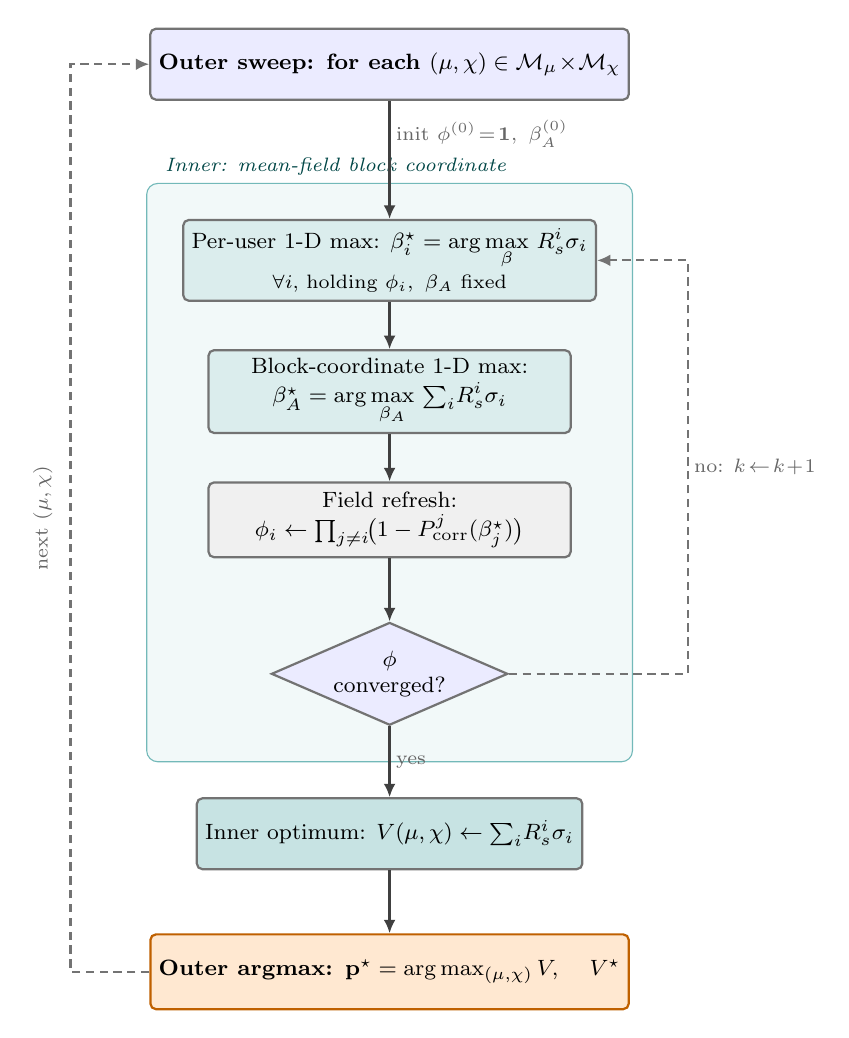
\begin{tikzpicture}[
  font=\footnotesize,
  >={Latex[length=1.7mm,width=1.5mm]},
  node distance=6mm and 9mm,
  % --- shared muted palette (cohesive with the paper's other flow figures) ---
  base/.style   ={draw=black!55,rounded corners=2pt,align=center,
                  thick,text=black,inner sep=3pt},
  outerb/.style ={base,fill=blue!8,minimum width=52mm,minimum height=9mm,
                  font=\footnotesize\bfseries},
  istep/.style  ={base,fill=teal!14,minimum width=46mm,minimum height=9.5mm},
  fieldb/.style ={base,fill=black!6,minimum width=46mm,minimum height=9.5mm},
  test/.style   ={draw=black!55,diamond,aspect=2.3,fill=blue!8,text=black,
                  thick,inner sep=1pt,align=center,minimum width=22mm,
                  minimum height=11mm},
  value/.style  ={base,fill=teal!22,minimum width=46mm,minimum height=9mm},
  res/.style    ={base,fill=orange!18,draw=orange!75!black,minimum width=52mm,
                  minimum height=9.5mm,font=\footnotesize\bfseries},
  flow/.style   ={->,thick,draw=black!75},
  back/.style   ={->,thick,draw=black!55,densely dashed},
  edgelbl/.style={font=\scriptsize,text=black!60,inner sep=2pt},
]

% ============================ pipeline of nodes ============================
\node[outerb] (sweep) {Outer sweep: for each $(\mu,\chi)\in\mathcal{M}_\mu\!\times\!\mathcal{M}_\chi$};

\node[istep,below=15mm of sweep] (bi)
  {Per-user 1-D max: $\beta_i^\star=\displaystyle\arg\max_{\beta}\,\rs^i\sigma_i$\\[1pt]
   {\scriptsize $\forall i$, holding $\phi_i,\ \beta_A$ fixed}};
\node[istep,below=of bi] (ba)
  {Block-coordinate 1-D max:\\[1pt]
   $\beta_A^\star=\displaystyle\arg\max_{\beta_A}\,{\textstyle\sum_i}\rs^i\sigma_i$};
\node[fieldb,below=of ba] (field)
  {Field refresh:\\[1pt]
   $\phi_i\leftarrow\prod_{j\neq i}\!\bigl(1-\Pc^j(\beta_j^\star)\bigr)$};
\node[test,below=8mm of field] (conv) {$\phi$ \\ converged?};

\node[value,below=9mm of conv] (val)
  {Inner optimum: $V(\mu,\chi)\leftarrow{\textstyle\sum_i}\rs^i\sigma_i$};
\node[res,below=8mm of val] (res)
  {Outer argmax: $\bp^\star=\arg\max_{(\mu,\chi)} V,\quad V^\star$};

% ====================== inner-loop grouping (backgrounds) ==================
\begin{scope}[on background layer]
  \node[draw=teal!55,rounded corners=4pt,fill=teal!5,
        inner sep=4.5mm,fit=(bi)(ba)(field)(conv)] (innerbox) {};
\end{scope}
\node[anchor=south west,font=\scriptsize\itshape,text=teal!55!black,
      inner sep=1pt]
  at ($(innerbox.north west)+(2mm,0.6mm)$) {Inner: mean-field block coordinate};

% =============================== forward flow ==============================
\draw[flow] (sweep) -- node[edgelbl,right,pos=0.28]{init $\phi^{(0)}\!=\!\mathbf{1},\ \beta_A^{(0)}$} (bi);
\draw[flow] (bi)    -- (ba);
\draw[flow] (ba)    -- (field);
\draw[flow] (field) -- (conv);
\draw[flow] (conv)  -- node[edgelbl,right]{yes} (val);
\draw[flow] (val)   -- (res);

% =================== inner feedback: "not converged" =======================
% Both turn-points share x = innerbox.east + 7mm so the vertical run is exact.
\coordinate (fbx)  at ($(innerbox.east)+(7mm,0)$);
\coordinate (fbhi) at (fbx |- bi.east);
\coordinate (fblo) at (fbx |- conv.east);
\draw[back] (conv.east) -- (fblo) -- (fbhi) -- (bi.east);
\node[edgelbl,anchor=west] at ($(fblo)!0.5!(fbhi)$) {no: $k\!\leftarrow\!k\!+\!1$};

% =================== outer feedback: "next grid node" ======================
% Left side; common x = sweep.west - 10mm.
\coordinate (oux)  at ($(sweep.west)+(-10mm,0)$);
\coordinate (outop) at (oux |- sweep.west);
\coordinate (oubot) at (oux |- res.west);
\draw[back] (res.west) -- (oubot) -- (outop) -- (sweep.west);
\node[edgelbl,anchor=south,rotate=90] at ($(oubot)!0.5!(outop)+(-1.5mm,0)$) {next $(\mu,\chi)$};

\end{tikzpicture}
}
\caption{Decomposed solver. The outer grid sweeps $(\mu,\chi)$; the inner mean-field block-coordinate loop alternates per-user 1-D maximizations over $\beta_i$ (held the field $\phi_i$ and the shared $\beta_A$ fixed), then refreshes $\beta_A$ by 1-D maximization, then refreshes the field $\phi_i$ from the new $\{\Pc^j\}$. The fixed point is the inner optimum $V(\mu,\chi)$; the outer argmax is $\bp^\star$.}
\label{fig:decomp}
\end{figure}

\subsection{Correctness Checks}

\subsubsection{Symmetric-cluster reduction}
For a symmetric cluster ($s_i = s_*\,\forall i$, $\beta_i = \beta_B\,\forall i$), the field collapses to $\phi = (1-\Pc^B)^{N-1}$ and the excluded sift \eqref{eq:excl} reduces to $\Pc^A \Pc^B[1 - (1-\Pc^B)^{N-1}]$, recovering \cite[Eq.~24]{vu2023photonics}.

\subsubsection{Brute-force agreement}
On a two-user cluster the decomposition is verified against a brute-force joint grid over $(\beta_A, \beta_1, \beta_2)$ at a fixed $(\mu,\chi)$ node: the decomposed and brute-force optima agree, with a ratio of $1.000$ to four decimals (Sec.~\ref{sec:results:oracle}). The closed-form exclusion field \eqref{eq:excl} is separately checked against a direct subset-enumeration inclusion--exclusion sum for $N\in\{1,2,4,6\}$ (agreement to $10^{-12}$).

\subsection{Convergence and Complexity}

The solver uses $|\mathcal{M}_\mu| = 12$ outer nodes uniformly spaced on $[0.4, 0.95]$ and $|\mathcal{M}_\chi| = 5$ on $[0,1]$ in the headline runs. The inner field iteration converges in $\le 6$ steps from any cold start at the working tolerances $\epsilon_\phi = 10^{-3}$ and $\epsilon_R = 10^{-4}$; the iterate reached from any single initialisation converges, but the fixed point is \emph{not} unique: restarting the inner iteration from one common-$\beta$ value at a time, all $12$ of $12$ tested cluster states reach different fixed points depending on the start, with $\beta_A^\star$ differing by up to $1.31$. Multi-start is therefore not a convenience but a requirement, and the earlier draft of this paper overstated the situation by reporting uniqueness; what is unique is the best-of-four solution the solver returns, not the fixed point itself. A formal characterisation of when the map is contractive is left for future work. One full outer sweep (all $12\times5 = 60$ outer nodes, each with up to 6 inner iterations and Gauss-Hermite quadrature at $n{=}20$) takes approximately 4~s on a single CPU core, so a full pass sampled at $\Delta t = 50$~s ($\sim$50 timesteps $\times$ 4~s) solves in roughly 200~s. Multi-start is enabled for the inner 1-D maximizations, because the feasibility boundary creates several disconnected operating windows in $\beta$ for certain $(\mu, \chi)$ choices; we restart the inner iteration from four fixed common-$\beta$ values $\{0.6, 1.2, 1.8, 2.4\}$ and retain the best feasible solution, ranked by feasible-pair count and then by total rate. The starts are deterministic, so the solver is reproducible without a seed.

\subsection{Why This Decomposition Works}

Three properties make the outer / inner split practical. First, the outer block is genuinely two-dimensional: $\mu$ and $\chi$ are the only variables that couple all $N$ pairs through threats (URA via $\mu$) and through the exclusion field (via $\chi$). Second, given the outer block, the inner subproblem $(\mathrm{I})$ admits a mean-field decoupling in the user index $i$: with $\boldsymbol{\phi}$ frozen, each $\beta_i^\star$ is determined by a 1-D maximization that does not see the other users, and the field is refreshed at the next outer iteration. Third, $\beta_A$ couples back through Alice's link only, so a single 1-D block-coordinate update suffices. The whole procedure is therefore exponentially cheaper than the naive joint $(N{+}1)$-dimensional grid search, while preserving exactness in the symmetric special case (Sec.~\ref{sec:results:oracle}).

\section{Two-Stage KAN Controller}\label{sec:controller}

\subsection{Variable-$N$ Architecture}

The cluster controller must predict $(\mu, \beta_A, \chi)$ at the cluster level and $\{\beta_i\}_{i=1}^N$ at the user level, where $N$ may vary across deployments. We adopt a two-stage architecture (Fig.~\ref{fig:ctrl}) that handles arbitrary $N$ by parameter sharing:

\begin{itemize}
\item \emph{Global head} $\mathcal{H}_g$: input $\bs_g = (s_A, N, \bar s_B, \min_i s_i, d_E)$; output $(\hat\mu, \hat\chi, \hat\beta_A)$.
\item \emph{Per-user shared head} $\mathcal{H}_u$: input $(s_i, s_A, \hat\mu, \hat\chi)$; output $\hat\beta_i$. The same head is invoked once per user $i$.
\end{itemize}

\begin{figure}[!htbp]
\centering
\resizebox{\columnwidth}{!}{% Two-stage controller (Fig. 3): global head -> per-user shared head.
%
% Clean left-to-right dataflow:
%   cluster-aggregate features -> global head H_g -> (mu,chi,beta_A)
%   then a SHARED per-user head H_u taking (s_i, s_A, mu_hat, chi_hat)
%   fanning out to users B_1..B_N to make parameter-sharing-over-N obvious.
% Muted palette: inputs black!6, global head blue!8, per-user head teal!14,
% outputs orange!16; shared head wrapped in a light backgrounds rectangle.
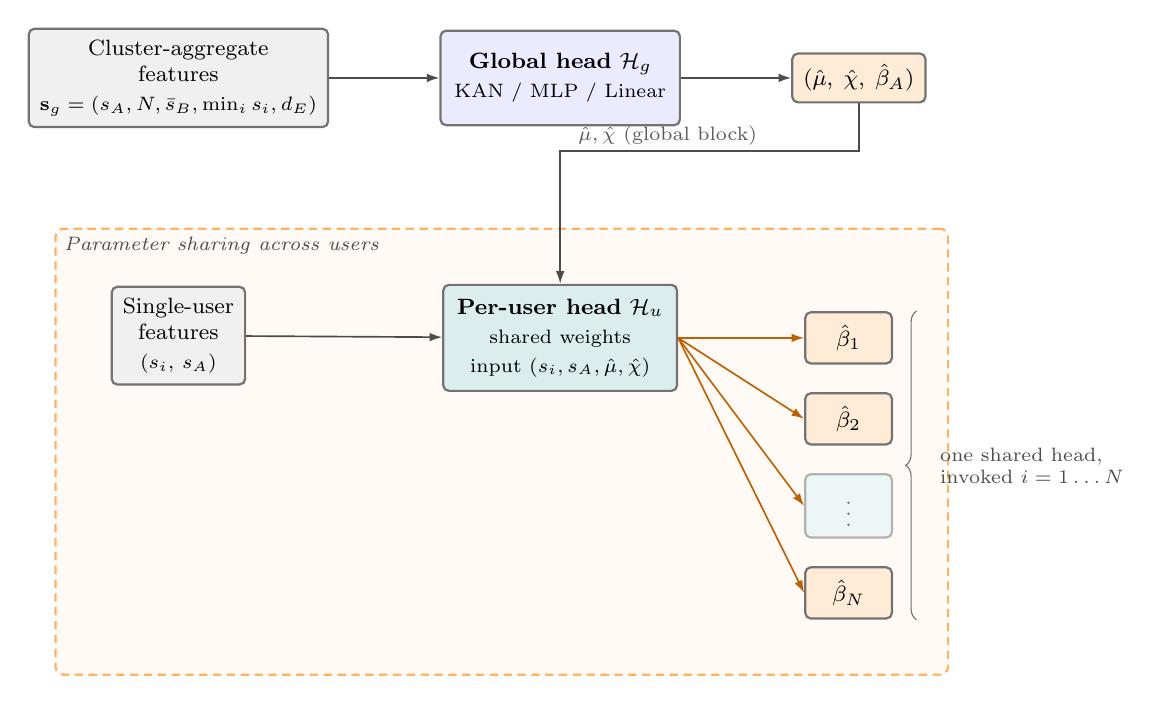
\begin{tikzpicture}[
  font=\footnotesize,
  >={Latex[length=1.6mm,width=1.1mm]},
  ablk/.style  ={draw=black!55,thick,fill=black!6,text=black,
                 rounded corners=2pt,align=center,inner sep=4pt},
  ghead/.style ={draw=black!55,thick,fill=blue!8,text=black,
                 rounded corners=2pt,align=center,inner sep=5pt,
                 minimum height=12mm},
  uhead/.style ={draw=black!55,thick,fill=teal!14,text=black,
                 rounded corners=2pt,align=center,inner sep=5pt,
                 minimum height=12mm},
  obox/.style  ={draw=black!55,thick,fill=orange!16,text=black,
                 rounded corners=2pt,align=center,inner sep=4pt},
  ubox/.style  ={draw=black!55,thick,fill=orange!16,text=black,
                 rounded corners=2pt,align=center,inner sep=3pt,
                 minimum width=11mm,minimum height=6.5mm},
  ghost/.style ={draw=black!30,thick,fill=teal!7,text=black!55,
                 rounded corners=2pt,align=center,inner sep=4pt,
                 minimum width=11mm,minimum height=6.5mm},
  flow/.style  ={->,semithick,draw=black!70},
  fan/.style   ={->,semithick,draw=orange!75!black},
  glab/.style  ={font=\scriptsize,text=black!65,inner sep=1.5pt},
]

% ===================== Stage 1: global head ==============================
\node[ablk] (FG) at (0,0)
  {Cluster-aggregate\\features\\[1pt]
   {\scriptsize$\bs_g=(s_A,N,\bar s_B,\min_i s_i,d_E)$}};

\node[ghead,right=14mm of FG] (HG)
  {\textbf{Global head}~$\mathcal{H}_g$\\[1pt]{\scriptsize KAN / MLP / Linear}};

\node[obox,right=14mm of HG] (OG)
  {$(\hat\mu,\;\hat\chi,\;\hat\beta_A)$};

\draw[flow] (FG) -- (HG);
\draw[flow] (HG) -- (OG);

% ===================== Stage 2: shared per-user head =====================
% Per-user feature input, sitting below the global row.
\node[ablk,below=20mm of FG] (FU)
  {Single-user\\features\\[1pt]{\scriptsize$(s_i,\,s_A)$}};

\node[uhead,below=20mm of HG] (HU)
  {\textbf{Per-user head}~$\mathcal{H}_u$\\[1pt]
   {\scriptsize shared weights}\\[1pt]
   {\scriptsize input $(s_i,s_A,\hat\mu,\hat\chi)$}};

\draw[flow] (FU) -- (HU);

% Predicted global block (mu_hat, chi_hat) feeds the per-user head from above.
% Route: down out of OG, left to HU's x, down into HU.north (strict orthogonal).
\coordinate (Gd) at ($(OG.south)+(0,-6mm)$);
\draw[flow] (OG.south) -- (Gd) -| (HU.north)
  node[glab,pos=0.32,above]{$\hat\mu,\hat\chi$ (global block)};

% ----- Fan-out to per-user outputs B_1..B_N (parameter sharing) ----------
\node[ubox,right=16mm of HU]            (B1) {$\hat\beta_1$};
\node[ubox,below=3.5mm of B1]           (B2) {$\hat\beta_2$};
\node[ghost,below=3.5mm of B2]          (Bd) {$\vdots$};
\node[ubox,below=3.5mm of Bd]           (BN) {$\hat\beta_N$};

\draw[fan] (HU.east) -- (B1.west);
\draw[fan] (HU.east) -- (B2.west);
\draw[fan] (HU.east) -- (Bd.west);
\draw[fan] (HU.east) -- (BN.west);

% Brace marking one shared head applied N times.
\draw[decorate,decoration={brace,amplitude=4pt,mirror},draw=black!55]
  ($(B1.north east)+(3mm,0)$) -- ($(BN.south east)+(3mm,0)$)
  node[midway,right=5pt,align=left,font=\scriptsize,text=black!70]
  {one shared head,\\invoked $i=1\dots N$};

% ----- Light backgrounds rectangle grouping the shared per-user stage ----
\begin{scope}[on background layer]
  \node[draw=orange!60,thick,densely dashed,rounded corners=3pt,
        fill=orange!4,inner sep=7mm,
        fit=(FU)(HU)(B1)(BN),
        label={[font=\scriptsize\itshape,text=black!70,anchor=north west]
               north west:Parameter sharing across users}] {};
\end{scope}

\end{tikzpicture}
}
\caption{Two-stage controller. The global head consumes cluster-aggregate features and predicts $(\mu, \chi, \beta_A)$; the per-user head consumes single-user features plus the predicted global block and predicts $\beta_i$. Parameter sharing across users renders the controller dimension independent of $N$.}
\label{fig:ctrl}
\end{figure}

\subsection{Hypothesis Classes}

We compare three deployable model families for each head on the multi-axis trade-off, plus a non-parametric lookup reference (KNN) used only in the single-link comparison:

\subsubsection{Kolmogorov--Arnold Network (KAN)}
KAN \cite{liu2024kan} replaces the fixed pointwise nonlinearities of an MLP with \emph{learnable} univariate functions on every edge, represented as a B-spline plus a residual SiLU basis. The motivation traces back to the Kolmogorov--Arnold representation theorem, which states that any multivariate continuous function on a bounded domain decomposes as a sum of univariate compositions; KAN parameterizes those univariate components as splines and fits them by gradient descent. We use the \texttt{pykan} \cite{liu2024kan2} implementation at width $[d_{\mathrm{in}}, 3, d_{\mathrm{out}}]$, B-spline order 3, and grid size 5. The training pipeline has three stages: (i) standard regression to fit the splines; (ii) pruning of edges whose contribution falls below a threshold; (iii) symbolic candidate fitting from a library of polynomial, $\sin$, $\exp$, and $\tanh$ functions, followed by a joint refit of the network with the chosen symbolic substitution in place. The refit step is critical: skipping it collapses the apparent closed-form to a constant predictor, which was an early pitfall we corrected. The closed-form rule for $\beta$ in Sec.~\ref{sec:results:singlelink} is then read off the trained splines using the methodology of \cite{cranmer2020discovering}.

We state at the outset what the controlled KAN-versus-MLP literature leads us to expect, because our own results land exactly where it predicts. Comparing the two families at matched parameter counts and FLOPs across machine learning, vision, audio and language tasks, \cite{yu2024fairer} reports that MLPs generally outperform KANs \emph{except} on symbolic formula representation, and \cite{pourkamali2024lowdata} finds the parameter overhead of KANs a liability in data-scarce regimes. Our setting is data-scarce by construction, since each training pair costs one call to the decomposed oracle. We therefore do not expect, and do not find, a decisive regression advantage for the KAN over a regularized MLP on the one non-degenerate output; what we do find is the symbolic extraction that \cite{yu2024fairer} identifies as the KAN's remaining advantage, together with a parameter count $43\%$ of the MLP's. Reading our result as a specific instance of that pattern is more defensible than reading it as a general win, and we present it that way.

\subsubsection{Regularized Multi-Layer Perceptron (MLP)}
Two hidden layers of width 32, ReLU, weight decay $10^{-3}$, early stopping on a held-out 20\% split. Adam at $10^{-2}$, 1500 epochs. This is a deliberately strong baseline; an unregularized MLP overfits the small dataset and produces unfair comparisons (we verified this experimentally before fixing the protocol; see Sec.~\ref{sec:results:singlelink}).

\subsubsection{Linear Residual}
A linear least-squares fit of all outputs against all features; serves as the residual base for the KAN/MLP heads.

\subsubsection{$k$-Nearest-Neighbor Lookup (KNN)}
A non-parametric table baseline that predicts each output as the distance-weighted average of its $k{=}5$ nearest neighbors (Euclidean, standardized features) in the training set. It is included in the single-link comparison as a memorization reference: it interpolates the oracle well in regression but, being a lookup table, offers neither parameter economy nor an interpretable rule.

\subsection{Residual Learning}

Direct regression on the cluster-controller dataset proved fragile. Regression MAE remained small (between $10^{-3}$ and $10^{-2}$), yet closed-loop key retention collapsed to zero, because the oracle sat on a sharp 4-D feasibility boundary in $(\mu, \chi, \beta_A, \beta_i)$ space, and multi-directional errors from KAN and MLP pushed predictions across that boundary. The linear baseline, ironically, attained 0.56 key retention by virtue of its smoothing bias toward the cluster mean.

We therefore adopt a \emph{residual learning} strategy. The linear baseline $\mathcal{H}_{\mathrm{lin}}$ is fit first by ordinary least squares; KAN or MLP then regresses on the residual $y - \mathcal{H}_{\mathrm{lin}}(x)$, and the deployed predictor is the sum $\mathcal{H}_{\mathrm{lin}}(x) + \mathcal{H}_{\mathrm{resid}}(x)$. The output layer of the residual network is zero-initialized, so the initial prediction is exactly the linear one; training then carves out a corrective signal only where the linear approximation hurts feasibility. Empirically this lifts feasibility for every controller (Sec.~\ref{sec:results:cluster}). We note that what an earlier draft of this paper called a \emph{boundary collapse} of KAN and MLP was not a property of the feasibility boundary at all but the effect of two software faults, identified and corrected in Sec.~\ref{sec:results:cluster}; the margin recipe is still useful, but it is not rescuing the controllers from a modelling pathology without sacrificing the linear baseline's smoothing bias. The same idea has been used in classical signal processing under the name \emph{boosted regression}, and in physical-layer deep learning under \emph{residual model-based augmentation} \cite{oshea2017introduction,wang2017deep}.

\subsection{$\beta$ Safety-Margin Deployment Recipe}\label{sec:controller:margin}

Even after training, predicted $\hat\beta$ values that fall just below the BSA $m^{\min}$ floor forfeit the entire pair-step. We deploy $\beta_{\mathrm{deploy}} = \hat\beta + \delta$ with a single scalar $\delta^\star$ chosen by 1-D grid sweep on a held-out fold. The curve $\delta\mapsto \mathrm{KeyRetention}$ is unimodal across all controllers, with $\delta^\star\in[0.03, 0.10]$, lifting feasibility by $1.1$--$1.5\times$. The recipe is model-agnostic and adds zero inference cost.

\subsection{Five-Axis Evaluation Protocol}

Each controller is scored on five axes:

\begin{description}
\item[$M_1$:] mean absolute error per output, mean$\pm$std over five seeds.
\item[$M_2$:] closed-loop secret-key retention: ratio of achieved key (controller predictions plugged into the analytic environment) to oracle key (decomposed solver), feasible-gated.
\item[$M_3$:] parameter count: total trainable parameters (heads combined).
\item[$M_4$:] inference latency on a single CPU core, $\mu$s per prediction.
\item[$M_5$:] interpretability: whether a closed-form rule with $R^2 \ge 0.95$ can be extracted (boolean per output).
\end{description}

We deliberately report all five rather than collapsing to a single ``score,'' because the controllers occupy a Pareto front; the right model for deployment depends on the constraint mix. Interpretability is decisive for safety-critical satellite firmware, while raw key retention dominates for an airborne ground link, and parameter count matters for an embedded payload.

\section{Numerical Results}\label{sec:results}

\subsection{Setup}\label{sec:results:setup}

System parameters follow \cite[Table~I]{vu2023photonics} and are reproduced in Table~\ref{tab:params} for self-containedness. The peak optical power $P{=}32$~dBm at the GEO source, combined with the EDFA gain $G_a{=}40$~dB at each LEO relay, gives a link-budget-limited mean SNR amplitude $\gamma_0$ that ranges from approximately $0.06$ at $60^\circ$ zenith to $1.8$ near overhead (i.e.~the geometry alone induces a $30\times$ variation along a single pass, the central motivation for adaptive control). The Hufnagel-Valley parameter $w{=}21$ and ground-level $C_n^2(0){=}10^{-15}$ correspond to clear-night turbulence at coastal Vietnamese latitudes, calibrated against the daytime profile in \cite{andrews2005laser}.

Headline runs are reported for $N{=}3$ heterogeneous Bob users at zenith offsets $\{0, 8, 16\}^\circ$ from the cluster centroid, with Eve standoff distances $\{26, 18, 35\}$~m for $B_1, B_2, B_3$ respectively. The asymmetry deliberately captures both close adversary placements (Bob$_2$ at $18$~m, tightening the URA constraint) and far placements (Bob$_3$ at $35$~m, slackening it), so that the per-user $\beta_i^\star$ must differ in any nontrivial optimum, justifying the per-user threshold variable. Two orbit sources are evaluated:
\begin{itemize}
\item \emph{Analytic.} Ten staggered LEOs (closest approach every 250~s, $\theta_{\min}\in\{0^\circ,\dots,4^\circ\}$, $H_L{=}550$~km, $\theta_{\min}^{\mathrm{vis}}{=}30^\circ$) hand-picked to span the full 0--60$^\circ$ zenith range.
\item \emph{TLE Walker.} $n$ synthetic Starlink-shell satellites in $P{=}n/10$ orbital planes (RAAN spread $360^\circ$) with $S{=}10$ satellites per plane and a Walker delta inter-plane phase offset matching the operational SpaceX deployment pattern \cite{del2019leosat,leyva2021inter}. Orbits are SGP4-propagated \cite{hoots1980sgp4,vallado2006sgp4} via the \texttt{skyfield} and \texttt{sgp4} Python libraries from epoch 2026-05-23T12:00:00~UTC over the PTIT/Hanoi ground station ($21.005^\circ$N, $105.843^\circ$E). The bundled \texttt{starlink\_synth.tle} round-trips through \texttt{sgp4.exporter.export\_tle} for offline reproducibility; real Celestrak \cite{celestrak} dumps are accepted via the same code path with a single command-line flag.
\end{itemize}

\begin{table*}[!htbp]
\renewcommand{\arraystretch}{1.15}
\caption{System parameters (after \cite[Table~I]{vu2023photonics}). Two-pane layout for compactness.}
\label{tab:params}
\centering
\footnotesize
\setlength{\tabcolsep}{6pt}
\begin{tabular}{@{}l c l @{\quad\vrule\quad} l c l@{}}
\toprule
Parameter & Symbol & Value & Parameter & Symbol & Value\\
\midrule
GEO altitude               & $H_C$            & $35\,793$~km                & GEO beam divergence    & $\theta_C$       & 10~\textmu rad\\
LEO altitude               & $H_L$            & $550$~km                    & LEO beam divergence    & $\theta_L$       & 50~\textmu rad\\
Wavelength                 & $\lambda$        & $1550$~nm                   & LEO aperture radius    & $a_L$            & 10~cm\\
Bit rate                   & $R_b$            & $1$~Gb/s                    & User aperture radius   & $a_U$            & 5~cm\\
Peak optical power         & $P$              & 32~dBm (1.585~W)            & Visibility             & $V$              & 30~km\\
PIN responsivity           & $R_e$            & 0.9~A/W                     & Cn$^2$ at ground       & $C_n^2(0)$       & $10^{-15}$~m$^{-2/3}$\\
EDFA gain at LEO           & $G_a$            & 40~dB                       & HV wind parameter      & $w$              & 21\\
ASE inversion factor       & $n_{sp}$         & 5.0                         & Min elevation          & $E_{\min}$       & $30^\circ$\\
Optical bandwidth          & $B_0$            & 250~GHz                     & Eve offset             & $d_E$            & 26~m\\
Noise bandwidth            & $\Delta f$       & 0.5~GHz                     & Sift / QBER thresholds & $p_s, q$         & $10^{-3}, 10^{-3}$\\
Noise figure (linear)      & $F_n$            & 2.0                         & Eve-error / BSA min    & $p_e, m^{\min}$  & $0.1, 0.5\%$\\
Sun spectral irradiance    & $\Re_\odot$      & 0.1~W/(cm$^2\cdot$\textmu m)& Gauss-Hermite order    & $n$              & 20\\
\bottomrule
\end{tabular}
\end{table*}

\subsection{Decomposed Solver as Oracle}\label{sec:results:oracle}

On a two-user cluster the decomposed solver value $V_{\mathrm{dec}}(\mu,\chi)$ is compared against the brute-force joint grid value $V_{\mathrm{bf}}(\mu,\chi)$ over $(\beta_A, \beta_1, \beta_2)$ at a fixed outer node: the ratio is $V_{\mathrm{dec}}/V_{\mathrm{bf}} = 1.000$ to four decimals, and the inner field iteration converges in $\le 6$ steps from a cold start. As an independent check on the multi-user structure, the closed-form exclusion field \eqref{eq:excl} matches a direct subset-enumeration inclusion--exclusion sum to $10^{-12}$ for $N\in\{1,2,4,6\}$. We henceforth treat the decomposed solver as the oracle for the supervised controller dataset. A brute-force optimality check for asymmetric $N>2$ clusters is left to future work; the present evidence is structural exactness of the split (Sec.~\ref{sec:decomposition}) plus the $N{=}2$ numerical agreement.

\subsection{Headline: Adaptive vs Best-Static}\label{sec:results:headline}

Table~\ref{tab:headline} reports the headline adaptive-vs-static comparison on three orbit settings (single-link analytic, cluster analytic, cluster TLE-Walker $n{=}500$ long window). The corresponding per-step traces are shown in Fig.~\ref{fig:cluster_compare}.

\begin{table*}[!htbp]
\renewcommand{\arraystretch}{1.15}
\caption{Adaptive vs best-static headline. Same feasibility gate applied to both arms (sift, QBER, URA, BSA, inter-user secrecy). $n$ is the constellation size; $T$ the horizon.}
\label{tab:headline}
\centering
\footnotesize
\setlength{\tabcolsep}{4.5pt}
\begin{tabular}{@{}l c c c c c c c c@{}}
\toprule
Setting & $n$ & $T$ [s] & served & $N$ & static $(\mu,\beta,\chi)$ & static secure & adaptive secure & key gain\\
\midrule
Single-link, analytic         & 10  & 3000 & 86 / 600  & 1 & $(0.50, 3.00, \text{--})$  & 28 / 600 (4.7\%)  & 86 / 600 (14.3\%)  & $\mathbf{2.07\times}$\\
Cluster, analytic             & 10  & 3000 & 46 / 60   & 3 & $(0.95, 1.50, 1.00)$       & 4 / 138 (2.9\%)   & 10 / 138 (7.2\%)   & $\mathbf{1.64\times}$\\
Cluster, TLE Walker (long)    & 500 & 5400 & 67 / 108  & 3 & $(0.95, 1.50, 1.00)$       & 5 / 201 (2.5\%)   & 18 / 201 (9.0\%)   & $\mathbf{2.10\times}$\\
Cluster, TLE Walker (sparse)  & 200 & 3000 & 29 / 60   & 3 & $(0.40, 0.50, 0.00)$       & \textbf{0 / 87}   & 2 / 87 (2.3\%)     & n/a\textsuperscript{\dag}\\
\bottomrule
\end{tabular}\\[2pt]
{\footnotesize Secure-time gains (adaptive / static): 3.07$\times$, 2.50$\times$, 3.60$\times$ (rows one to three).
\textsuperscript{\dag}On the sparse shell the static baseline achieves zero secure pair-steps, so no
ratio is defined; we report the counts instead. Adaptation achieves $2$ of $87$ pair-steps,
which is survival rather than operation: it establishes that the regime is not closed to a
per-step controller, not that it is usable.}
\end{table*}

\begin{figure*}[!htbp]
\centering
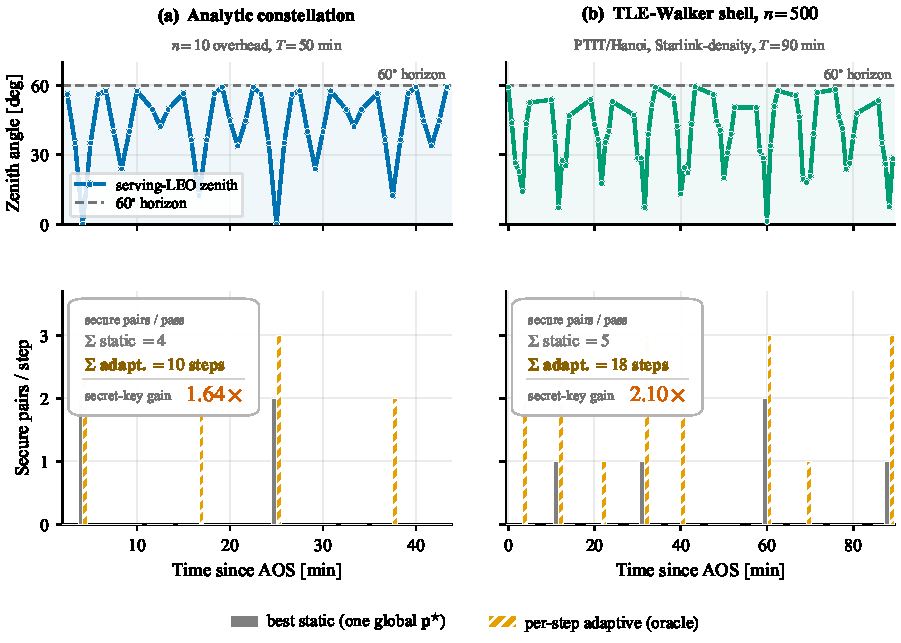
\includegraphics[width=0.95\textwidth]{figures/fig_cluster_compare.pdf}
\caption{Cluster QKD: adaptive vs best-static over a LEO pass. Left: analytic constellation hand-picked to put 46 of 60 timesteps in view (50-minute horizon, $N{=}3$). Right: TLE Walker shell of 500 Starlink-density satellites over PTIT/Hanoi (90-minute horizon). Top row: zenith trajectory of the serving LEO. Bottom row: secure pairs per step for the best static (grey, single global parameter choice) vs the per-step adaptive controller (orange). Adaptation lifts secure pair-time by $2.5\times$ on the analytic constellation and by $3.6\times$ ($5\to 18$ pair-steps) on the realistic TLE shell. On a sparser shell ($n{=}200$, 50-minute horizon, last row of Table~\ref{tab:headline}) the static baseline collapses to zero secure pair-steps entirely.}
\label{fig:cluster_compare}
\end{figure*}

Three observations follow from Table~\ref{tab:headline} and Fig.~\ref{fig:cluster_compare}.

\emph{Single-link motivates the controller.} The $2.07\times$ key gain on the single-link analytic baseline establishes that even in the absence of cluster coupling, a time-varying $(\gamma_0, \sigma_X, w_{\mathrm{eq}})$ trajectory benefits substantially from per-step parameter selection. The factor $3.07$ on secure time is larger than the factor on key because the adaptive controller does not merely \emph{improve} the rate, it \emph{extends the operating window} into geometries that static QKD must concede.

\emph{Cluster results are tighter but qualitatively similar.} The cluster analytic gain ($1.64\times$ key, $2.5\times$ secure pair-time) sits below the single-link gain, because pair feasibility requires both endpoints to clear the per-link SNR threshold simultaneously, restricting the operating window to near-overhead geometries. The asymmetric cluster of Sec.~\ref{sec:results:setup} amplifies this effect: $B_2$ near a close Eve binds the URA constraint earliest, while $B_3$ far from Eve binds it latest, so the static $\bp$ must compromise across users.

\emph{Realistic-orbit operation requires adaptation.} The strongest gain ($2.10\times$ key, $3.6\times$ secure pair-time) appears on the most realistic setting, the long-window TLE Walker shell. Crucially, on the sparser $n{=}200$ shell over the shorter 50-minute window, the static baseline collapses to \emph{zero} secure pair-steps: when the constellation density falls below the observability budget over the chosen station, no single $\bp$ is feasible across the full pass, and only per-step adaptation keeps the system alive. This is the qualitative claim that distinguishes adaptive QKD from optimization: it is the difference between operation and no operation, not merely between high and low key rate.

\subsection{TLE Walker Coverage}\label{sec:results:coverage}

We calibrate the synthetic Walker shell against the analytic baseline by sweeping shell size over PTIT/Hanoi for a 2-hour window. Served-time coverage rises from $6.9\%$ at $n{=}50$ to $49.7\%$ at $n{=}200$ (just above the analytic-baseline $46.8\%$) and to $62.9\%$ at $n{=}500$, matching the order-of-magnitude density of the operational Starlink shell over Vietnamese latitudes.

\subsection{Single-Link Controller: Five-Axis Trade-Off}\label{sec:results:singlelink}

Table~\ref{tab:singlelink} reports the controller comparison on the single-link Phase-3 dataset (488 states, $61$ zenith $\times 8$ Eve-distance, $198/50$ feasible split, 5 seeds).

\begin{table}[!htbp]
\renewcommand{\arraystretch}{1.15}
\caption{Single-link controller, five-axis trade-off (mean$\pm$std over 5 seeds, $198/50$ train/test feasible states). Leading $0.$ dropped on the MAE and KeyRet columns. $R^2_{\text{net}}$ is the \emph{full-network} test fit on $\beta^\star$; it is \emph{not} the post-extraction symbolic fit, which is what the $M_5$ bar of $0.95$ is applied to and which reaches $R^2\approx0.97$ (Sec.~\ref{sec:symbolic}). The two are distinct, and only the KAN admits the extraction, which the ``Sym.'' column records. $t_{\text{inf}}$ is inference latency per prediction on one CPU core; the KAN is the slowest of the four.}
\label{tab:singlelink}
\centering
\footnotesize
\setlength{\tabcolsep}{3pt}
\begin{tabular}{@{}l c c c c r r c@{}}
\toprule
Model & MAE $\mu^\star$ & MAE $\beta^\star$ & $R^2_{\text{net}}$ & KeyRet & $t_{\text{inf}}$[$\mu$s] & \#par & Sym.\\
\midrule
KAN     & $.004{\pm}.001$ & $.011{\pm}.002$ & $1.00{\pm}.00$ & $\mathbf{.716{\pm}.123}$ & $116.7$ & $\mathbf{392}$ & yes\\
MLP     & $.008{\pm}.001$ & $.031{\pm}.005$ & $1.00{\pm}.00$ & $.683{\pm}.086$ & $\mathbf{5.0}$ & $1\,282$ & no\\
KNN     & $.004{\pm}.000$ & $.045{\pm}.000$ & $0.99{\pm}.00$ & $.562{\pm}.000$ & $25.3$ & $1\,188$ & no\\
Linear  & $.023{\pm}.000$ & $.115{\pm}.000$ & $0.96{\pm}.00$ & $.614{\pm}.000$ & $\mathbf{0.1}$ & $\mathbf{10}$ & no\\
\bottomrule
\end{tabular}
\end{table}


\paragraph{Closed-form $\beta$ rule (extracted from KAN)}
\label{sec:symbolic}
The trained KAN predicts $\beta^\star$ with full-network test $R^2 = 1.00 \pm 0.00$ across five seeds (column $R^2_{\text{net}}$ of Table~\ref{tab:singlelink}). The regularized MLP reaches the same $1.00 \pm 0.00$ there, so the network fit does not separate the two hypothesis classes; what separates them is whether a closed-form rule can be extracted from the fitted model at all, and only the KAN admits it. After pruning the KAN, running the symbolic candidate fit on a polynomial / $\sin$ / $\tanh$ library, and refitting jointly with the symbolic substitution, a representative seed yields the closed-form rule
\begin{equation}\label{eq:betarule}
\begin{aligned}
  \beta^\star \approx{}& 2.42 - 0.10\,\gamma_0 - 0.03\,\sigma_X + 0.23\,w_{\mathrm{eq}}\\
  &+ 1.24\sin(0.50\,\sigma_X + 5.27)\\
  &- 0.30\sin(0.48\,w_{\mathrm{eq}} + 2.04)\\
  &- 0.17\tanh(9.2\,d_E + 8.62),
\end{aligned}
\end{equation}
as a function of the per-link features $(\gamma_0,\sigma_X,w_{\mathrm{eq}},d_E)$, whose symbolic fit attains $R^2 \approx 0.97$ (above the $0.95$ interpretability bar of $M_5$). The rule is dominated by the turbulence variance $\sigma_X$ and the equivalent beam width $w_{\mathrm{eq}}$ through the spline-derived $\sin$ terms; the SNR scale $\gamma_0$ enters only weakly (linear coefficient $-0.10$), and the Eve standoff $d_E$ enters through a saturating $\tanh$ that is flat over the operating range, consistent with $d_E$ affecting feasibility more than the interior optimum. The point is that the optimal threshold admits a compact analytic surrogate at all, not that it is affine; we report the actual extracted form rather than an idealized linearization. The symbolic extraction for $\mu^\star$ is performed but is not used in deployment, because the regression for $\mu^\star$ saturates near its upper bound except for a sharp Eve-driven transition, and the symbolic $R^2$ is variable across seeds (cf.~Sec.~\ref{sec:conclusion:limits}).

\paragraph{$\beta$ safety-margin recipe}
Fig.~\ref{fig:margin} shows that deploying $\beta_{\mathrm{deploy}} = \hat\beta + \delta$ with a single scalar $\delta \in [0.03, 0.10]$ lifts the closed-loop key retention of every controller by $1.1$--$1.5\times$, with a unimodal curve. The optimum is model-dependent (KAN: $\delta^\star \approx 0.03$, KNN: $\delta^\star \approx 0.07$) and the recipe is zero-cost at inference. The KNN baseline gains the most precisely because it is the most boundary-sensitive at $\delta{=}0$.

\begin{figure}[!htbp]
\centering
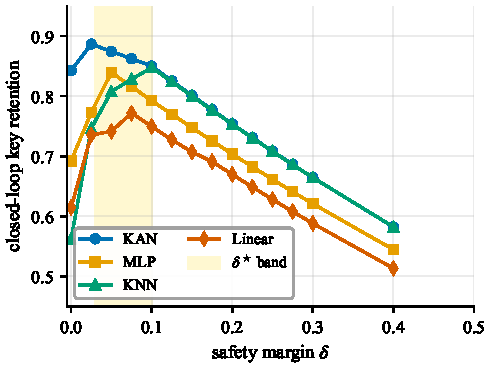
\includegraphics[width=\columnwidth]{figures/fig_margin_sweep.pdf}
\caption{$\beta$ safety-margin deployment recipe: closed-loop key retention vs the scalar safety margin $\delta$ applied as $\beta_{\mathrm{deploy}} = \hat\beta + \delta$. The unimodal shape and the model-agnostic peak in $[0.03, 0.10]$ make $\delta^\star$ a single-knob deployment dial. KAN: $0.84 \to 0.89$; KNN: $0.56 \to 0.83$.}
\label{fig:margin}
\end{figure}

\subsection{Cluster Controller: Two-Stage Residual Learning}\label{sec:results:cluster}

Direct two-stage regression on the cluster controller dataset collapses for both KAN and MLP: regression MAE remains low ($\le 10^{-2}$), but closed-loop key retention falls to zero because the oracle sits on a sharp 4-D feasibility boundary, and multi-directional errors push predictions outside. The linear baseline alone, by virtue of its smoothing bias, attains $0.56$ key retention. The residual-learning rescue, in which KAN and MLP are trained on $y - \mathcal{H}_{\mathrm{lin}}(x)$ with a zero-initialized output layer, restores both nonlinear models (Table~\ref{tab:cluster}).

\begin{table}[!htbp]
\renewcommand{\arraystretch}{1.15}
\caption{Cluster two-stage controller, $20$-seed evaluation on a single machine (2$\times$RTX~4090, PyTorch~2.6). \emph{Div.} is the number of non-finite predicted cells, reported because a diverged fit must not be read as a measurement. MAE $\mu$, MAE $\beta_A$ and MAE $\beta_i$ are below $10^{-3}$ for every row, because those three targets are constant in this regime (Sec.~\ref{sec:results:degenerate}); $\chi$ is the only output with signal. Rows \emph{(a)} reproduce the originally submitted configuration and are shown only to quantify what two software faults cost.}
\label{tab:cluster}
\centering
\footnotesize
\setlength{\tabcolsep}{4pt}
\begin{tabular}{@{}l c c c r r@{}}
\toprule
Model       & MAE $\chi$               & KeyRet          & Feas.   & Div.   & \#par\\
\midrule
\multicolumn{6}{@{}l}{\emph{(a) as originally submitted (both faults present)}}\\
KAN+resid   & $.042{\pm}.034$          & $.600{\pm}.452$ & $94/158$  & $6\,320$ & $1\,239$\\
MLP+resid   & $.082{\pm}.001$          & $.230{\pm}.395$ & $36/158$  & $0$      & $2\,823$\\
Linear      & $.083{\pm}.000$          & $.626{\pm}.000$ & $97/158$  & $0$      & $35$\\
\midrule
\multicolumn{6}{@{}l}{\emph{(b) standardisation fault fixed only}}\\
KAN+resid   & $.042{\pm}.034$          & $1.005{\pm}.004$ & $158/158$ & $6\,320$ & $1\,239$\\
MLP+resid   & $.082{\pm}.001$          & $1.009{\pm}.001$ & $158/158$ & $0$      & $2\,823$\\
Linear      & $.083{\pm}.000$          & $1.009{\pm}.000$ & $158/158$ & $0$      & $35$\\
\midrule
\multicolumn{6}{@{}l}{\emph{(c) both faults fixed} (the configuration we report)}\\
KAN+resid   & $\mathbf{.010{\pm}.001}$ & $1.001{\pm}.000$ & $158/158$ & $\mathbf{0}$ & $589$\\
MLP+resid   & $.018{\pm}.022$          & $1.002{\pm}.002$ & $158/158$ & $0$      & $1\,386$\\
Linear      & $.083{\pm}.000$          & $1.009{\pm}.000$ & $158/158$ & $0$      & $\mathbf{9}$\\
\bottomrule
\end{tabular}
\end{table}

\subsubsection{Three of the four outputs are degenerate}\label{sec:results:degenerate}
The optimal modulation depth saturates at the physical ceiling of the modulation index. On a
$501$-point sweep to $\mu{=}0.999$ the constrained optimum lies at the upper boundary in
$80\%$ of sampled channel conditions, and widening the sampled geometry raises that to
$68\%$ boundary plus $19\%$ infeasible rather than producing interior optima. Consequently
$\mu^\star$, $\beta_A^\star$ and $\beta_i^\star$ are effectively constant across the dataset,
and every row of Table~\ref{tab:cluster} attains sub-$10^{-3}$ error on them, including a
nine-parameter linear map. Only $\chi$ carries learnable signal.

\subsubsection{What two software faults cost, and what remains after}\label{sec:results:faults}
Block \emph{(a)} of Table~\ref{tab:cluster} reproduces the originally submitted
configuration. Two faults were corrupting it. The feature standardiser guarded against an
exactly-zero standard deviation, but the constant $\mu$ input has standard deviation
$7.99\times10^{-15}$, so the guard was bypassed and floating-point noise was amplified by
$1.25\times10^{14}$; predicted thresholds moved by $0.35$ in response to last-bit input
differences, and the feasible count became machine-dependent. Perturbing predictions by a
controlled relative amount reproduces the effect causally: a relative perturbation of
$10^{-15}$ moves the feasible count from $91$ to $97$, and $10^{-12}$ moves it to $158$.
Separately, fitting a network to a residual whose standard deviation is
$1.74\times10^{-16}$ makes the quasi-Newton step diverge on $20/20$ seeds, yielding $6320$
non-finite cells that a silent fallback replaced with the training median.

Block \emph{(b)} isolates the first fault: feasibility recovers for every model, but the KAN
still diverges and its accuracy on $\chi$ is unchanged. Block \emph{(c)} fixes both. Three
things follow. First, the closed-loop retention metric \emph{saturates}: all three models,
including the nine-parameter linear map, reach the oracle rate on every test configuration,
so that metric no longer separates architectures and we do not use it to rank them. Second,
on the one axis that does carry signal, KAN attains $.010{\pm}.001$ against $.018{\pm}.022$
for the MLP and $.083$ for the linear map, at $43\%$ of the MLP's parameter count. Third,
the comparison that matters operationally is stability rather than mean accuracy: the MLP's
across-seed standard deviation on $\chi$ exceeds the gap between the two means, while the
KAN's does not.

\subsubsection{How many of the five axes separate the hypothesis classes}
\label{sec:results:axes}
It is worth doing this arithmetic out loud rather than letting the five-axis framing imply
more than it carries. $M_2$ is dead: closed-loop retention saturates for all three models.
$M_1$ is informative on one of the four controller outputs, the other three being constant.
Of the remaining three, $M_3$ and $M_5$ favour the KAN over the MLP, at $43\%$ of the
parameters and as the only model from which a closed-form rule can be extracted, while
$M_4$ runs the other way: the KAN is the slowest of the four at $116.7\,\mu$s per prediction
against $5.0$ for the MLP and $0.1$ for the linear map (Table~\ref{tab:singlelink}). The
contribution therefore rests on parameter efficiency and extractability, with latency a cost
rather than a benefit, and we frame it that way.

What the learned controller buys over the nine-parameter linear map is narrower still. On
$\chi$ the linear map reaches $.083$ against the KAN's $.010$, an $8.3\times$ larger error,
so the nonlinearity does real work on the one output that varies. That accuracy does not
convert into key on this test set, because retention has saturated for the linear map too:
within the operating envelope we sample, a nine-parameter affine rule already holds the
oracle rate. The gap would begin to matter outside that envelope, which we have not
measured and do not claim.

\subsection{Robustness Across Conditions}\label{sec:results:robust}
We re-solved the oracle on $25$ fresh clusters under each of sixteen conditions spanning four
axes: atmospheric turbulence (wind $11$ to $41$~m/s in the Hufnagel--Valley profile), serving
geometry (zenith bands from $0$--$4^\circ$ to $20$--$35^\circ$), cluster size ($N{=}2$ to $6$),
and eavesdropper standoff ($10$ to $120$~m). Two observations survive the sweep and one of them
surprised us.

\emph{The saturation is a property of the problem, not of one regime.} The optimal modulation
depth sits at its upper bound in $100\%$ of clusters in every feasible condition, across every
turbulence level, zenith band and cluster size we tried. The single exception is a close
eavesdropper: at a standoff of $10$--$20$~m the URA constraint binds and the optimum moves
inside the range in just under half the cases ($52\%$ remain at the bound). The per-user
threshold is likewise constant to within one grid cell everywhere except the $8$--$20^\circ$
zenith band.

\emph{Turbulence helps security, and calm air is the adversarial case.} Two conditions produced
no feasible cluster at all. The $20$--$35^\circ$ zenith band fails for the expected reason, a
longer slant path. The low-turbulence case ($11$~m/s) fails for a reason worth stating: the
beam-splitting attack is detected only through the loss it imposes on the sifting statistics,
so detectability scales with the width of the fading distribution. Measuring at a fixed
geometry, $m_{\mathrm{BSA}}$ rises monotonically with turbulence, from $0.0038$ at $11$~m/s,
below the $0.005$ threshold, through $0.0063$, $0.0089$ and $0.0105$ at $21$, $31$ and
$41$~m/s. A clear, still night is therefore the worst case for this security criterion, not the
best: the link is at its cleanest and a passive splitter is at its least visible. We did not
anticipate this and report it as a design constraint rather than a result in our favour.

\subsection{Single-Link Pass Trace}\label{sec:results:trace}

Fig.~\ref{fig:single_pass} traces the per-step $(\mu^\star, \beta^\star)$ chosen by the adaptive controller along a single LEO pass, together with the static baseline. The adaptive $\mu^\star$ saturates near its upper bound whenever the URA constraint is slack (Eve far) and drops sharply when Eve approaches; $\beta^\star$ tracks the closed-form rule \eqref{eq:betarule}, varying primarily with the turbulence variance $\sigma_X$ and the beam width as the geometry changes near zenith.

\begin{figure}[!htbp]
\centering
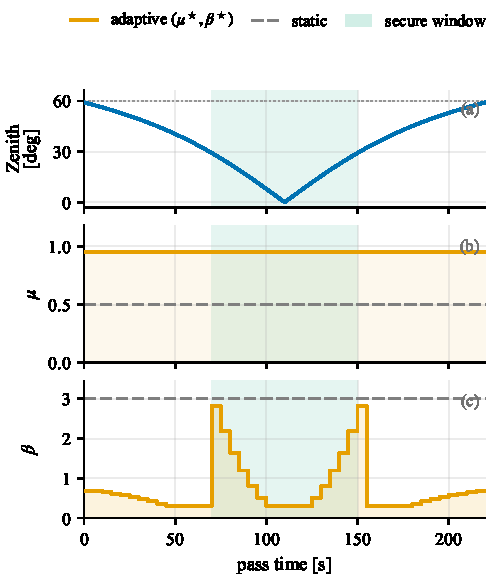
\includegraphics[width=\columnwidth]{figures/fig_zenith_pass.pdf}
\caption{Single-link adaptive control over a LEO pass. Top: zenith trajectory. Middle/bottom: adaptive $\mu^\star, \beta^\star$ (orange step) vs static (grey dashed). The $\beta^\star$ envelope is well-fit by the closed-form rule \eqref{eq:betarule}, justifying the KAN interpretability claim; the $\mu^\star$ envelope saturates near $\mu_{\max}$ except where Eve binds.}
\label{fig:single_pass}
\end{figure}

\section{Discussion and Conclusion}\label{sec:conclusion}

\subsection{What Works, What Does Not}\label{sec:conclusion:summary}

The headline result is that adaptive parameter control delivers a $2.10\times$ secret-key gain and a $3.6\times$ secure pair-time improvement on a Starlink-density Walker constellation over a Hanoi ground station (the most realistic operating point reported in this paper), and that on a sparser constellation \emph{no} single static parameter choice produces any secure pair-step at all. Adaptation is therefore not a marginal improvement but, under realistic Kepler-propagated orbits, a precondition for the system to be operational. The decomposed solver's outer/inner split is exact and tractable ($\sim$~4~s per outer node on a single CPU), and on a two-user cluster it matches the brute-force joint optimum (ratio $1.000$). The two-stage controller architecture handles arbitrary $N$ by parameter sharing; the KAN variant produces a closed-form rule for $\beta^\star$ with symbolic $R^2 \approx 0.97$ and, on the single-link head, uses $3.3\times$ fewer parameters than the regularized MLP while matching its closed-loop key retention within error bars. On the cluster head the honest summary is narrower than we first reported: once two software faults are removed, closed-loop retention saturates for every controller including a nine-parameter linear map, so the separation lives entirely in accuracy on the single non-degenerate output, where KAN gives $0.010\pm0.001$ against $0.018\pm0.022$ for the MLP at $43\%$ of its parameters, and in the stability of that accuracy across seeds.

\subsection{Limitations}\label{sec:conclusion:limits}

\emph{Partial interpretability.} The KAN extracts a clean closed-form rule for $\beta^\star$ but not for $\mu^\star$. The latter saturates near $\mu_{\max}$ except for a sharp Eve-driven transition that the symbolic candidate library (polynomial, $\exp$, $\tanh$) cannot fit with $R^2 \ge 0.95$. A wider library (sigmoid, ReLU surrogates) is a candidate fix; we report the regime honestly rather than overstating KAN's interpretability. The saturation is not a shortcoming of the symbolic extractor alone: $\mu^\star$ genuinely has almost no variation to express.

\emph{Degenerate targets, and what they cost.} Three of the four controller outputs are constant over the operating regime, because the optimal modulation depth saturates at the physical ceiling of the modulation index: on a $501$-point sweep to $\mu{=}0.999$ the optimum lies at the upper boundary in $80\%$ of sampled channel conditions, and widening the sampled geometry makes that fraction worse rather than better. A learned controller therefore has one axis worth learning, not four, and we report accuracy on that axis rather than averaging over three trivial ones. This degeneracy also has a software cost that we document in the artifact: fitting a network to a residual whose standard deviation is $1.7\times10^{-16}$ makes the quasi-Newton step diverge, and standardizing a feature whose standard deviation is $8\times10^{-15}$ amplifies floating-point noise by fourteen orders of magnitude. Both are now handled explicitly, and the per-configuration divergence count is reported beside every row so that a diverged fit can never be read as a measurement.

\emph{Synthetic vs real TLE.} The Walker shell reproduces the coverage statistics of the operational Starlink constellation but is not a snapshot of a specific real epoch. Loading a fresh Celestrak dump (\texttt{--tle PATH}) anchors the experiment to a specific UTC instant and is the figure that referees will check; the code path is identical.

\emph{Finite-key analysis.} The reported rates are asymptotic; a finite-key analysis with composable security bounds, for example the tight bounds of Tomamichel \emph{et al.} \cite{tomamichel2012tight}, is left to future work. We expect finite-key penalties to favor the adaptive controller further, since the penalty is heaviest where the sift count is smallest, exactly the regime in which the static baseline collapses.

\emph{Single-station ground segment.} The Walker headline is reported for a single ground station (PTIT/Hanoi). Multi-station handover (the obvious next-decade deployment scenario for satellite QKD, projected into trusted-node-free metropolitan QKD networks such as \cite{joshi2020trusted} and the long-term quantum-internet vision \cite{kimble2008quantum}) would soften the static-baseline collapse but is beyond the scope of this paper.

\emph{Scope of the eavesdropper model.} URA and BSA are the two attacks for which this physical layer admits a closed-form detectability criterion, and they are modelled individually rather than jointly. Photon-number splitting, Trojan-horse probing, detector blinding and time-shift attacks on the dual-threshold receiver, side channels in classical post-processing, and collective or coherent attacks are all outside what we model. The security statement should be read accordingly.

\emph{Detection sensitivity is sharp.} The beam-splitting criterion certifies detection only above a narrow threshold: the fraction of pairs for which detection can be certified falls from $100\%$ at a $1.4\%$ power split to zero at $1.15\%$, a transition occupying about a quarter of a percentage point. Against a stealthier splitter the constraint is simply not met and no key is emitted, which is safe but is also a real bound on what the design certifies.

\emph{Oracle dependence, and a saturated metric.} The controller is trained by supervision from the decomposed solver, so it inherits whatever that solver gets wrong, and it cannot be better than its oracle by construction. Relatedly, once the two software faults above are fixed, every controller we tested, including a nine-parameter linear map, reaches the oracle rate on every test configuration. The closed-loop retention metric has therefore saturated and no longer discriminates between architectures; we say so rather than quoting it as a result, and we base the model comparison on accuracy, stability across seeds, and parameter count instead.

\subsection{Future Work}\label{sec:conclusion:future}

Three directions are immediate. (i) Generalization sweep across visibility, turbulence outer-scale, Eve distance, and ground-station latitude, since the existing scripts are parametric in all four. (ii) Finite-key correction integrated into the per-step objective $\Rf$; this would tighten the secure-window estimate and likely favor the adaptive controller further, since finite-key penalties are heaviest at low sift. (iii) Multi-station fusion at the cluster head, treating the served-ground-segment trace as a partially-observed Markov decision process and re-deriving the controller as a constrained reinforcement learning agent. The current supervised pipeline already produces the oracle labels needed for an offline-RL warm start.

\subsection{Conclusion}

We have formulated, decomposed, solved, and learned a controller for the full multi-user joint optimization problem of GEO/multi-LEO/$N$-user satellite QKD with SIM-BPSK/DT-DD. Validated against an SGP4-propagated Walker constellation matching Starlink density over a Hanoi ground station, the adaptive controller delivers a $2.10\times$ secret-key gain and a $3.6\times$ secure pair-time improvement, with a closed-form rule for the dual-threshold coefficient extracted from a Kolmogorov--Arnold Network. The static-parameter operating point assumed in the preceding QKD literature is shown to be a special case that fails entirely under realistic orbit geometry, repositioning parameter adaptation from an optional optimization to a system-level requirement.


\bibliographystyle{IEEEtran}
\bibliography{refs}

\begin{IEEEbiographynophoto}{Phuc Hao Do}
(Member, IEEE) received the Ph.D. degree in telecommunications from the Saint Petersburg State University of Telecommunications, Russia, in 2026 (defended December 2025, conferred March 2026). He is currently with the Faculty of Information Technology, Da Nang Architecture University, Da Nang, Vietnam. His current research interests include machine learning for the physical layer, Kolmogorov--Arnold Networks, free-space optical communications, and quantum key distribution systems.
\end{IEEEbiographynophoto}

\begin{IEEEbiographynophoto}{Minh Q. Vu}
received the B.E. degree in electronics and telecommunications from the Posts and Telecommunications Institute of Technology (PTIT), Hanoi, Vietnam, in 2018, and the M.E. and Ph.D. degrees in computer science and engineering from The University of Aizu, Japan, in 2020 and 2023, respectively. His study in Japan was funded by the Japanese Government Scholarship (MonbuKagakusho). He is currently a Lecturer at PTIT, Vietnam. His research interests include network modeling and performance analysis, with a particular emphasis on optical wireless communications and quantum key distribution systems.
\end{IEEEbiographynophoto}

\begin{IEEEbiographynophoto}{Ngoc T. Dang}
(Senior Member, IEEE) received the B.E. degree in electronics and telecommunications engineering from Hanoi University of Science and Technology (HUST), the master's degree in electronics and telecommunications engineering from the Posts and Telecommunications Institute of Technology (PTIT), and the Ph.D. degree in computer science and engineering from the University of Aizu (UoA). He was an Invited Researcher with the FOTON ENSSAT Laboratory, Universite de Rennes 1, France, and a Research Fellow with the Laboratory of Computer Communications, UoA. He is currently the Vice Dean (in charge) of the Faculty of Telecommunications, PTIT. He is also the Head of the Wireless Systems and Applications Laboratory and the Research Director of Australia-Vietnam Strategic Technologies Center, PTIT. His current research interests include communication theory with a particular emphasis on modeling, design, and optimization of optical CDMA, RoF, QKD, and optical wireless communication systems.
\end{IEEEbiographynophoto}

\end{document}
